\clearpage

\phantomsection

\setcounter{chapter}{3}
\chapter[{THỰC NGHIỆM VÀ ĐÁNH GIÁ}]{THỰC NGHIỆM VÀ ĐÁNH GIÁ}

Chương này trình bày toàn bộ quá trình thực nghiệm của hệ thống AnimeGANv3 (DTGAN) được xây dựng trong luận văn, bao gồm: mô tả môi trường phần cứng và phần mềm, bộ dữ liệu sử dụng, nghi thức đánh giá, phân tích đường cong hội tụ huấn luyện, đánh giá định lượng bằng các chỉ số FID và LPIPS, đánh giá định tính trên cả ba chế độ (Face Mode, Landscape Mode, Hybrid Mode), đánh giá riêng cho module Face Mode, khảo sát cảm nhận người dùng, và cuối cùng là ứng dụng web triển khai hệ thống.

Các phân tích trong chương được đặt trong mối liên hệ với những dự đoán lý thuyết đã nêu ở Chương~2 và Chương~3, nhằm kiểm chứng xem các lập luận thiết kế có được thực nghiệm xác nhận hay không.

% =====================================================
\section{Môi trường Thực nghiệm}
\label{sec:exp_env}

\subsection{Cấu hình Phần cứng}
\label{subsec:hardware}

Toàn bộ quá trình huấn luyện và thực nghiệm được thực hiện trên nền tảng điện toán đám mây chuyên biệt cho AI \textbf{vast.ai} với cấu hình máy chủ như sau:

\begin{table}[H]
\caption{Cấu hình phần cứng sử dụng trong thực nghiệm}
\label{tab:hardware}
\centering
\begin{tabular}{|p{3.5cm}|p{11.5cm}|}
\hline
\textbf{Thành phần} & \textbf{Thông số} \\
\hline
GPU & \textbf{1x NVIDIA RTX A5000} (Workstation/Server) \newline - VRAM: 24 GB GDDR6 \newline - Hiệu năng: 27,5 TFLOPS \newline - Băng thông bộ nhớ: 650,8 GB/s \\
\hline
CPU & \textbf{Intel Core i9-10900X} (sử dụng 10 nhân / 20 luồng) \\
\hline
RAM & \textbf{64 GB} khả dụng (trên tổng số 129 GB của máy chủ) \\
\hline
Lưu trữ & \textbf{SSD MSI M482 2TB} (tốc độ đọc/ghi $\approx$ 3090 MB/s) \newline - Dung lượng trống cấp phát: 711,5 GB \\
\hline
Mạng & \textbf{Băng thông}: Upload 776 Mbps / Download 802 Mbps \\
\hline
\end{tabular}
\end{table}

%%% CẦN KIỂM TRA: bản gốc có dòng "CUDA hỗ trợ tối đa: 13.2" đã được tạm gỡ bỏ
%%% vì mâu thuẫn với "CUDA Toolkit 10.0" khai báo ở Bảng phần mềm bên dưới.
%%% Hãy xác nhận lại phiên bản CUDA/driver thực tế trên máy chủ vast.ai đã dùng
%%% và bổ sung lại dòng này nếu cần.

Cấu hình trên được lựa chọn dựa trên hai ràng buộc chính. Thứ nhất, dung lượng VRAM 24~GB là mức tối thiểu cần thiết để chứa đồng thời Generator hai nhánh, hai Discriminator và mạng VGG19 đóng băng phục vụ Content Loss và Style Loss (Chương~2, Mục~\ref{sec:loss}) --- đây cũng là lý do batch size bị giới hạn ở mức 8. Thứ hai, CPU nhiều nhân là yêu cầu bắt buộc chứ không phải tùy chọn: như đã phân tích ở Chương~2 (Mục~\ref{subsec:training_stages}), thuật toán Felzenszwalb superpixel và NL-Means + L0 Smoothing chạy trên CPU song song với forward pass trên GPU; nếu CPU không đủ nhanh, GPU sẽ phải chờ và toàn bộ lợi ích của việc chồng lấp thời gian bị mất.

\subsection{Cấu hình Phần mềm}
\label{subsec:software}

\begin{table}[H]
\caption{Cấu hình phần mềm và thư viện sử dụng}
\label{tab:software}
\centering
\begin{tabular}{|p{4.5cm}|p{10.5cm}|}
\hline
\textbf{Thành phần} & \textbf{Phiên bản / Môi trường} \\
\hline
Môi trường huấn luyện & Docker Image \texttt{vastai/tensorflow} (trên \textbf{vast.ai}) \\
\hline
Hệ điều hành & Ubuntu 16.04 LTS (Server) / Windows 10 (Local) \\
\hline
Python & 3.6.x (trên vast.ai) / 3.7.x (Local) \\
\hline
TensorFlow & 1.12.0rc1 \\
\hline
CUDA Toolkit & 10.0 \\
\hline
cuDNN & 7 \\
\hline
ONNX Runtime & 1.13.1 \\
\hline
Backend API Server & FastAPI \\
\hline
Frontend Web UI & React 19 \\
\hline
Thư viện xử lý ảnh & OpenCV 4.5.x, Pillow 8.x, scikit-image 0.18.x \\
\hline
\end{tabular}
\end{table}

%%% CẦN KIỂM TRA: cặp (TensorFlow 1.12 + CUDA 10.0) và GPU RTX A5000 (kiến trúc
%%% Ampere, compute capability 8.6) không tương thích theo tài liệu chính thức
%%% của NVIDIA -- Ampere yêu cầu CUDA >= 11. Hãy xác nhận lại phiên bản thực tế
%%% bên trong Docker image vastai/tensorflow đã sử dụng, hoặc ghi rõ nếu đã dùng
%%% bản TensorFlow do NVIDIA biên dịch lại (nvcr.io/nvidia/tensorflow).
%%% Đây là chi tiết hội đồng rất dễ đặt câu hỏi.

Việc hệ thống sử dụng \textbf{hai môi trường tách biệt} --- TensorFlow 1.x cho huấn luyện và ONNX Runtime cho suy luận --- là một quyết định kiến trúc quan trọng đã được đề cập ở Chương~3 (Mục~\ref{subsec:normalize_inference}). Mô hình sau khi huấn luyện được xuất sang định dạng ONNX, nhờ đó ứng dụng triển khai hoàn toàn không phụ thuộc vào TensorFlow --- một framework đã ngừng hỗ trợ và rất khó cài đặt trên môi trường Python hiện đại. Đây là điều kiện tiên quyết để ứng dụng web có thể chạy trên máy chủ thông thường.

% =====================================================
\section{Bộ Dữ liệu}
\label{sec:dataset}

\subsection{Dữ liệu Ảnh Thực (Photo)}
\label{subsec:photo_data}

Tập dữ liệu ảnh thực dùng cho huấn luyện bao gồm ảnh chân dung từ nhiều nguồn, mang tính đa dạng cao về giới tính, độ tuổi, sắc tộc và điều kiện ánh sáng: tập \textit{train\_photo} dùng chung với \textbf{6.656 ảnh}, và tập \texttt{train/images} của Ghibli\_o1 với \textbf{4.991 ảnh}. Toàn bộ tập ảnh đã được chọn lọc nhằm loại bỏ các trường hợp quá mờ, quá tối hoặc không có khuôn mặt nổi bật. Trước khi đưa vào mô hình, kích thước mỗi ảnh được chuẩn hóa về $256 \times 256$ (đối với cả chế độ Landscape và Face Mode).

Ở bước tiền xử lý, hệ thống tạo thêm một tập dữ liệu phụ mang tên \texttt{seg\_train\_5-0.8-50/}. Tập dữ liệu này chứa các ảnh đã qua phân mảnh bề mặt bằng thuật toán Felzenszwalb superpixel segmentation (với tham số $\sigma=5$, $k=0{,}8$ và $\text{min\_size}=50$), được sử dụng chuyên biệt để phục vụ việc tính toán thành phần Region Smoothing Loss trong quá trình huấn luyện (Chương~2, Mục~\ref{subsec:region_loss}).

\subsection{Dữ liệu Ảnh Anime (Style)}
\label{subsec:anime_data}

Dữ liệu phong cách anime được trích xuất từ phim hoạt hình của các đạo diễn nổi tiếng và được chia thành ba tập chính:
\begin{itemize}
    \item \textbf{Hayao Miyazaki (1.792 ảnh):} Các frame từ phim \textit{Spirited Away}, \textit{My Neighbor Totoro} --- phong cách ấm áp (warm), giàu màu sắc tự nhiên, đường nét mềm mại. Chủ yếu là phong cảnh (landscape). Không ghép cặp.
    \item \textbf{Makoto Shinkai (1.650 ảnh):} Các frame từ \textit{Your Name}, \textit{Weathering With You} --- phong cách lạnh, ánh sáng cinematic, chi tiết mịn. Chủ yếu là phong cảnh (landscape). Không ghép cặp.
    \item \textbf{Ghibli\_o1 (4.991 cặp ảnh):} Tập dữ liệu chuyên biệt về chân dung (portrait), bao gồm \texttt{train/images} (ảnh thực) và \texttt{train/gt} (ground-truth anime tương ứng). Tính chất ghép cặp (paired) giúp cung cấp tín hiệu giám sát mạnh mẽ cho việc học chi tiết khuôn mặt.
\end{itemize}

Mỗi tập anime không ghép cặp (Hayao, Shinkai) đi kèm tập \texttt{smooth/} được tạo bằng Edge Smoothing --- làm mờ nhẹ vùng biên trong ảnh anime, phục vụ số hạng thứ ba trong hàm mất mát của Support Discriminator (Chương~2, Phương trình~\ref{eq:disc_support_loss}).

\begin{table}[H]
\caption{Tóm tắt ba tập dữ liệu phong cách sử dụng trong luận văn}
\label{tab:dataset_summary}
\centering
\begin{tabular}{|l|c|c|c|p{4cm}|}
\hline
\textbf{Tập dữ liệu} & \textbf{Số ảnh} & \textbf{Ghép cặp} & \textbf{Nội dung chính} & \textbf{Đặc trưng phong cách} \\
\hline
Hayao Miyazaki & 1.792 & Không & Phong cảnh & Tông ấm, nét mềm \\
\hline
Makoto Shinkai & 1.650 & Không & Phong cảnh & Tông lạnh, ánh sáng cinematic \\
\hline
Ghibli\_o1 & 4.991 & Có & Chân dung & Giám sát trực tiếp chi tiết mặt \\
\hline
\end{tabular}
\end{table}

\medskip
\noindent\textit{\textbf{Nhận xét về đặc điểm dữ liệu:} Ba tập dữ liệu có sự chênh lệch đáng chú ý về bản chất, và điều này ảnh hưởng trực tiếp tới kết quả. Hai tập Hayao và Shinkai chủ yếu là \textbf{phong cảnh} và \textbf{không ghép cặp} --- tức mô hình phải học phong cách chân dung từ dữ liệu hầu như không chứa chân dung, chỉ thông qua tín hiệu đối kháng gián tiếp. Ngược lại, Ghibli\_o1 là tập \textbf{chân dung ghép cặp}, cung cấp giám sát trực tiếp cho đúng bài toán mà luận văn hướng tới. Vì vậy, có cơ sở để kỳ vọng chất lượng chuyển đổi khuôn mặt trên Ghibli\_o1 vượt trội hai tập còn lại, và mức chênh lệch này chính là một đại lượng đáng đo đạc. Luận văn ghi nhận đây là một hướng phân tích chưa được thực hiện đầy đủ trong phạm vi thực nghiệm hiện tại --- các chỉ số định lượng ở Mục~\ref{sec:quantitative} được báo cáo trên một cấu hình huấn luyện, chưa tách theo từng tập phong cách. Bổ sung bảng so sánh FID theo ba tập dữ liệu là công việc nên được ưu tiên trong lần thực nghiệm tiếp theo.}

\subsection{Lưu ý về Bản quyền và Đạo đức}
\label{subsec:copyright}

Toàn bộ các ảnh anime và frame cắt từ phim có bản quyền thuộc Studio Ghibli (\textit{Ghibli\_o1} và \textit{Hayao}) cũng như CoMix Wave Films (\textit{Shinkai}) là tài sản sở hữu trí tuệ độc quyền của tác giả và chủ sở hữu bản quyền tương ứng. Trong phạm vi luận văn này, các tập dữ liệu trên chỉ được sử dụng nghiêm ngặt cho mục đích nghiên cứu học thuật phi thương mại và đánh giá thuật toán theo nguyên tắc sử dụng hợp lý (fair use), và không được phân phối lại cho các ứng dụng thương mại.

Về phía dữ liệu ảnh chân dung người thật, các nguyên tắc xử lý dữ liệu sinh trắc học đã được nêu tại Chương~3 (Mục~\ref{subsec:privacy}) được áp dụng nhất quán trong toàn bộ quá trình thực nghiệm.

% =====================================================
\section{Nghi thức Đánh giá}
\label{sec:protocol}

Mục này xác định rõ các chỉ số và nghi thức đo được sử dụng trong toàn chương. Việc trình bày tách bạch nghi thức trước khi báo cáo kết quả nhằm đảm bảo các con số ở các mục sau được diễn giải đúng và có thể tái lập.

\subsection{Các Chỉ số Đánh giá}
\label{subsec:metrics}

\begin{table}[H]
\caption{Tóm tắt các chỉ số đánh giá định lượng sử dụng trong thực nghiệm}
\label{tab:metrics_desc}
\centering
\begin{tabular}{|p{2.5cm}|p{4cm}|p{7cm}|}
\hline
\textbf{Chỉ số} & \textbf{Tên đầy đủ} & \textbf{Ý nghĩa} \\
\hline
FID $\downarrow$ & Fréchet Inception Distance & Khoảng cách giữa phân phối đặc trưng của ảnh sinh và của ảnh anime thật --- càng thấp càng giống phong cách đích \cite{Heusel2017} \\
\hline
LPIPS & Learned Perceptual Image Patch Similarity & Khác biệt tri giác giữa ảnh đầu vào và ảnh đầu ra --- đo mức \textit{bảo toàn nội dung} \cite{Zhang2018LPIPS} \\
\hline
FPS $\uparrow$ & Frames Per Second & Số ảnh xử lý được mỗi giây --- đo hiệu năng suy luận \\
\hline
Kích thước model & -- & Dung lượng file ONNX (MB) \\
\hline
\end{tabular}
\end{table}

\subsubsection{Fréchet Inception Distance (FID)}

FID \cite{Heusel2017} đo khoảng cách giữa hai phân phối ảnh bằng cách xấp xỉ mỗi phân phối bằng một phân phối Gauss nhiều chiều trong không gian đặc trưng của mạng Inception-v3:

\begin{equation}
\label{eq:fid}
\text{FID}(r, g) = \underbrace{\left\| \mu_r - \mu_g \right\|_2^2}_{\text{(1) khác biệt về vị trí}} + \underbrace{\text{Tr}\!\left( \Sigma_r + \Sigma_g - 2\left(\Sigma_r \Sigma_g\right)^{1/2} \right)}_{\text{(2) khác biệt về hình dạng phân phối}}
\end{equation}

\noindent trong đó:
\begin{itemize}
    \item $(\mu_r, \Sigma_r)$ --- vector trung bình và ma trận hiệp phương sai của đặc trưng Inception-v3 (tầng \texttt{pool3}, 2048 chiều) trên tập ảnh \textit{thật}.
    \item $(\mu_g, \Sigma_g)$ --- các đại lượng tương ứng trên tập ảnh \textit{sinh ra}.
    \item $\text{Tr}(\cdot)$ --- vết ma trận (tổng các phần tử trên đường chéo chính).
\end{itemize}

\textbf{Ý nghĩa từng số hạng:} Số hạng (1) phạt sự lệch nhau về đặc trưng trung bình --- tương ứng với việc ảnh sinh ra có ``chất'' tổng thể khác ảnh thật. Số hạng (2) phạt sự khác biệt về mức độ đa dạng và cấu trúc tương quan giữa các đặc trưng --- đây là thành phần nhạy với hiện tượng sụp đổ mode (mode collapse), khi mô hình sinh ra nhiều ảnh gần giống nhau và $\Sigma_g$ trở nên suy biến so với $\Sigma_r$. FID bằng 0 khi và chỉ khi hai phân phối Gauss xấp xỉ trùng khớp hoàn toàn.

\subsubsection{Learned Perceptual Image Patch Similarity (LPIPS)}

LPIPS \cite{Zhang2018LPIPS} đo sự khác biệt tri giác giữa hai ảnh bằng cách so sánh đặc trưng sâu tại nhiều tầng của mạng VGG hoặc AlexNet:

\begin{equation}
\label{eq:lpips}
d(x, x_0) = \sum_{l} \frac{1}{H_l W_l} \sum_{h,w} \left\| w_l \odot \left( \hat{\phi}_l^{hw}(x) - \hat{\phi}_l^{hw}(x_0) \right) \right\|_2^2
\end{equation}

\noindent trong đó $\hat{\phi}_l^{hw}$ là đặc trưng đã chuẩn hóa theo kênh tại tầng $l$, vị trí $(h, w)$ của mạng tri giác, $w_l$ là vector trọng số được học cho tầng $l$, và $\odot$ là phép nhân theo từng phần tử.

\textbf{Lưu ý quan trọng về cách diễn giải.} Khác với FID, \textbf{LPIPS không phải là chỉ số ``càng thấp càng tốt'' một cách vô điều kiện}. Trong luận văn này, LPIPS được đo giữa \textit{ảnh đầu vào} và \textit{ảnh đầu ra}, nên nó phản ánh mức độ \textbf{bảo toàn nội dung} chứ không phải chất lượng phong cách. Điều này dẫn tới hai hệ quả cần ghi nhớ:

\begin{itemize}
    \item Một mô hình trả về nguyên vẹn ảnh đầu vào (phép đồng nhất) sẽ đạt $\text{LPIPS} = 0$ --- giá trị ``tốt nhất'' có thể --- nhưng hoàn toàn vô dụng cho bài toán anime hóa.
    \item Ngược lại, LPIPS quá cao cho thấy ảnh đầu ra đã đi quá xa khỏi ảnh gốc, làm mất đặc điểm nhận dạng của chủ thể.
\end{itemize}

Vì vậy, LPIPS chỉ nên được đọc \textbf{cùng với} FID, và chỉ có ý nghĩa khi so sánh các phương pháp có mức độ phong cách hóa tương đương. Một cặp giá trị lý tưởng là \textit{FID thấp} (đúng phong cách anime) đi kèm \textit{LPIPS ở mức vừa phải} (vẫn nhận ra người trong ảnh). Cách hiểu này khác với ký hiệu mũi tên $\downarrow$ thường thấy trong các bảng so sánh, và luận văn chủ động không dùng ký hiệu đó cho LPIPS nhằm tránh gây hiểu nhầm.

\subsection{Nghi thức Đo}
\label{subsec:eval_protocol}

Để kết quả có thể tái lập, nghi thức đo được cố định như sau:

\begin{itemize}
    \item \textbf{Tập đánh giá:} 1.000 ảnh chân dung, tách riêng hoàn toàn khỏi tập huấn luyện.
    \item \textbf{Tập tham chiếu cho FID:} tập ảnh anime thật tương ứng với phong cách đích.
    \item \textbf{Mạng đặc trưng:} Inception-v3 (\texttt{pool3}, 2048 chiều) cho FID; VGG cho LPIPS.
    \item \textbf{Môi trường suy luận:} ONNX Runtime, GPU RTX A5000.
    \item \textbf{Đo tốc độ:} lấy trung bình sau khi bỏ qua 10 lần chạy khởi động (warm-up), nhằm loại trừ chi phí khởi tạo phiên và biên dịch kernel lần đầu.
\end{itemize}

%%% CẦN ĐIỀN/XÁC NHẬN:
%%%  - Nguồn của 1.000 ảnh chân dung dùng làm tập đánh giá (bộ dữ liệu nào?)
%%%  - Số lượng và nguồn ảnh anime thật dùng làm tập tham chiếu FID
%%%  - Số lần chạy warm-up và số lần lặp khi đo FPS (nếu khác với con số nêu trên)
%%% Hội đồng thường hỏi rất kỹ phần này; nếu thiếu, kết quả FID không thể tái lập.

\subsection{Lưu ý về Tính So sánh được giữa các Chế độ}
\label{subsec:comparability}

Có một điểm phương pháp luận cần được nêu rõ trước khi trình bày kết quả. Ba chế độ vận hành của hệ thống sinh ra ảnh đầu ra thuộc \textbf{các miền ảnh khác nhau}:

\begin{itemize}
    \item \textbf{Face Mode} cho đầu ra là \textit{vùng khuôn mặt} kích thước $256\times256$.
    \item \textbf{Landscape Mode} cho đầu ra là \textit{toàn bộ ảnh} ở kích thước gốc.
    \item \textbf{Hybrid Mode} cho đầu ra là \textit{toàn bộ ảnh}, trong đó vùng khuôn mặt đã được thay thế.
\end{itemize}

Vì FID đo khoảng cách giữa hai \textit{phân phối ảnh}, việc so sánh trực tiếp FID của ảnh khuôn mặt cắt riêng với FID của ảnh toàn cảnh là \textbf{không hợp lệ về mặt thống kê}: hai tập ảnh có nội dung, bố cục và độ đa dạng khác hẳn nhau, nên chênh lệch FID sẽ phản ánh sự khác biệt về miền ảnh chứ không phải chênh lệch về chất lượng mô hình.

Để loại bỏ nguy cơ này, các chỉ số FID và LPIPS báo cáo tại Mục~\ref{sec:quantitative} được đo trên một \textbf{vùng đánh giá thống nhất} cho cả ba chế độ: với mỗi ảnh trong tập đánh giá, vùng khuôn mặt sau Margin Expansion được xác định một lần duy nhất, sau đó cắt ra từ đầu ra của \textit{cả ba} chế độ và đưa vào tính toán. Nhờ vậy, mọi chế độ đều được chấm điểm trên cùng một loại nội dung và chênh lệch quan sát được phản ánh đúng năng lực xử lý khuôn mặt.

%%% RẤT QUAN TRỌNG -- CẦN XÁC NHẬN:
%%% Đoạn trên mô tả nghi thức ĐÚNG cần dùng. Hãy đối chiếu với cách bạn đã đo thực tế:
%%%  (a) Nếu bạn ĐÃ đo FID trên cùng vùng khuôn mặt cho cả 3 chế độ -> giữ nguyên đoạn này.
%%%  (b) Nếu bạn đo FID của Face Mode trên ảnh crop, còn Landscape/Hybrid trên ảnh đầy đủ
%%%      -> cần ĐO LẠI theo nghi thức trên, hoặc sửa đoạn này và hạ giọng tuyên bố
%%%      "cải thiện 8,7%" thành "FID trên vùng khuôn mặt", đồng thời sửa cả Chương 3 và Chương 5.
%%% Đây là câu hỏi mà hội đồng nhiều khả năng sẽ đặt ra.

% =====================================================
\section{Kết quả Huấn luyện}
\label{sec:training_results}

\subsection{Giai đoạn Pre-training Generator}
\label{subsec:pretrain_results}

Trong giai đoạn pre-training (5 epoch đầu, tương ứng 2.080 steps với 416 steps/epoch), chỉ Generator được huấn luyện với Content Loss thuần túy (không có Discriminator). Hình~\ref{fig:pretrain_loss} cho thấy đường cong hội tụ của Pre-train G\_loss:

\begin{figure}[H]
    \centering
    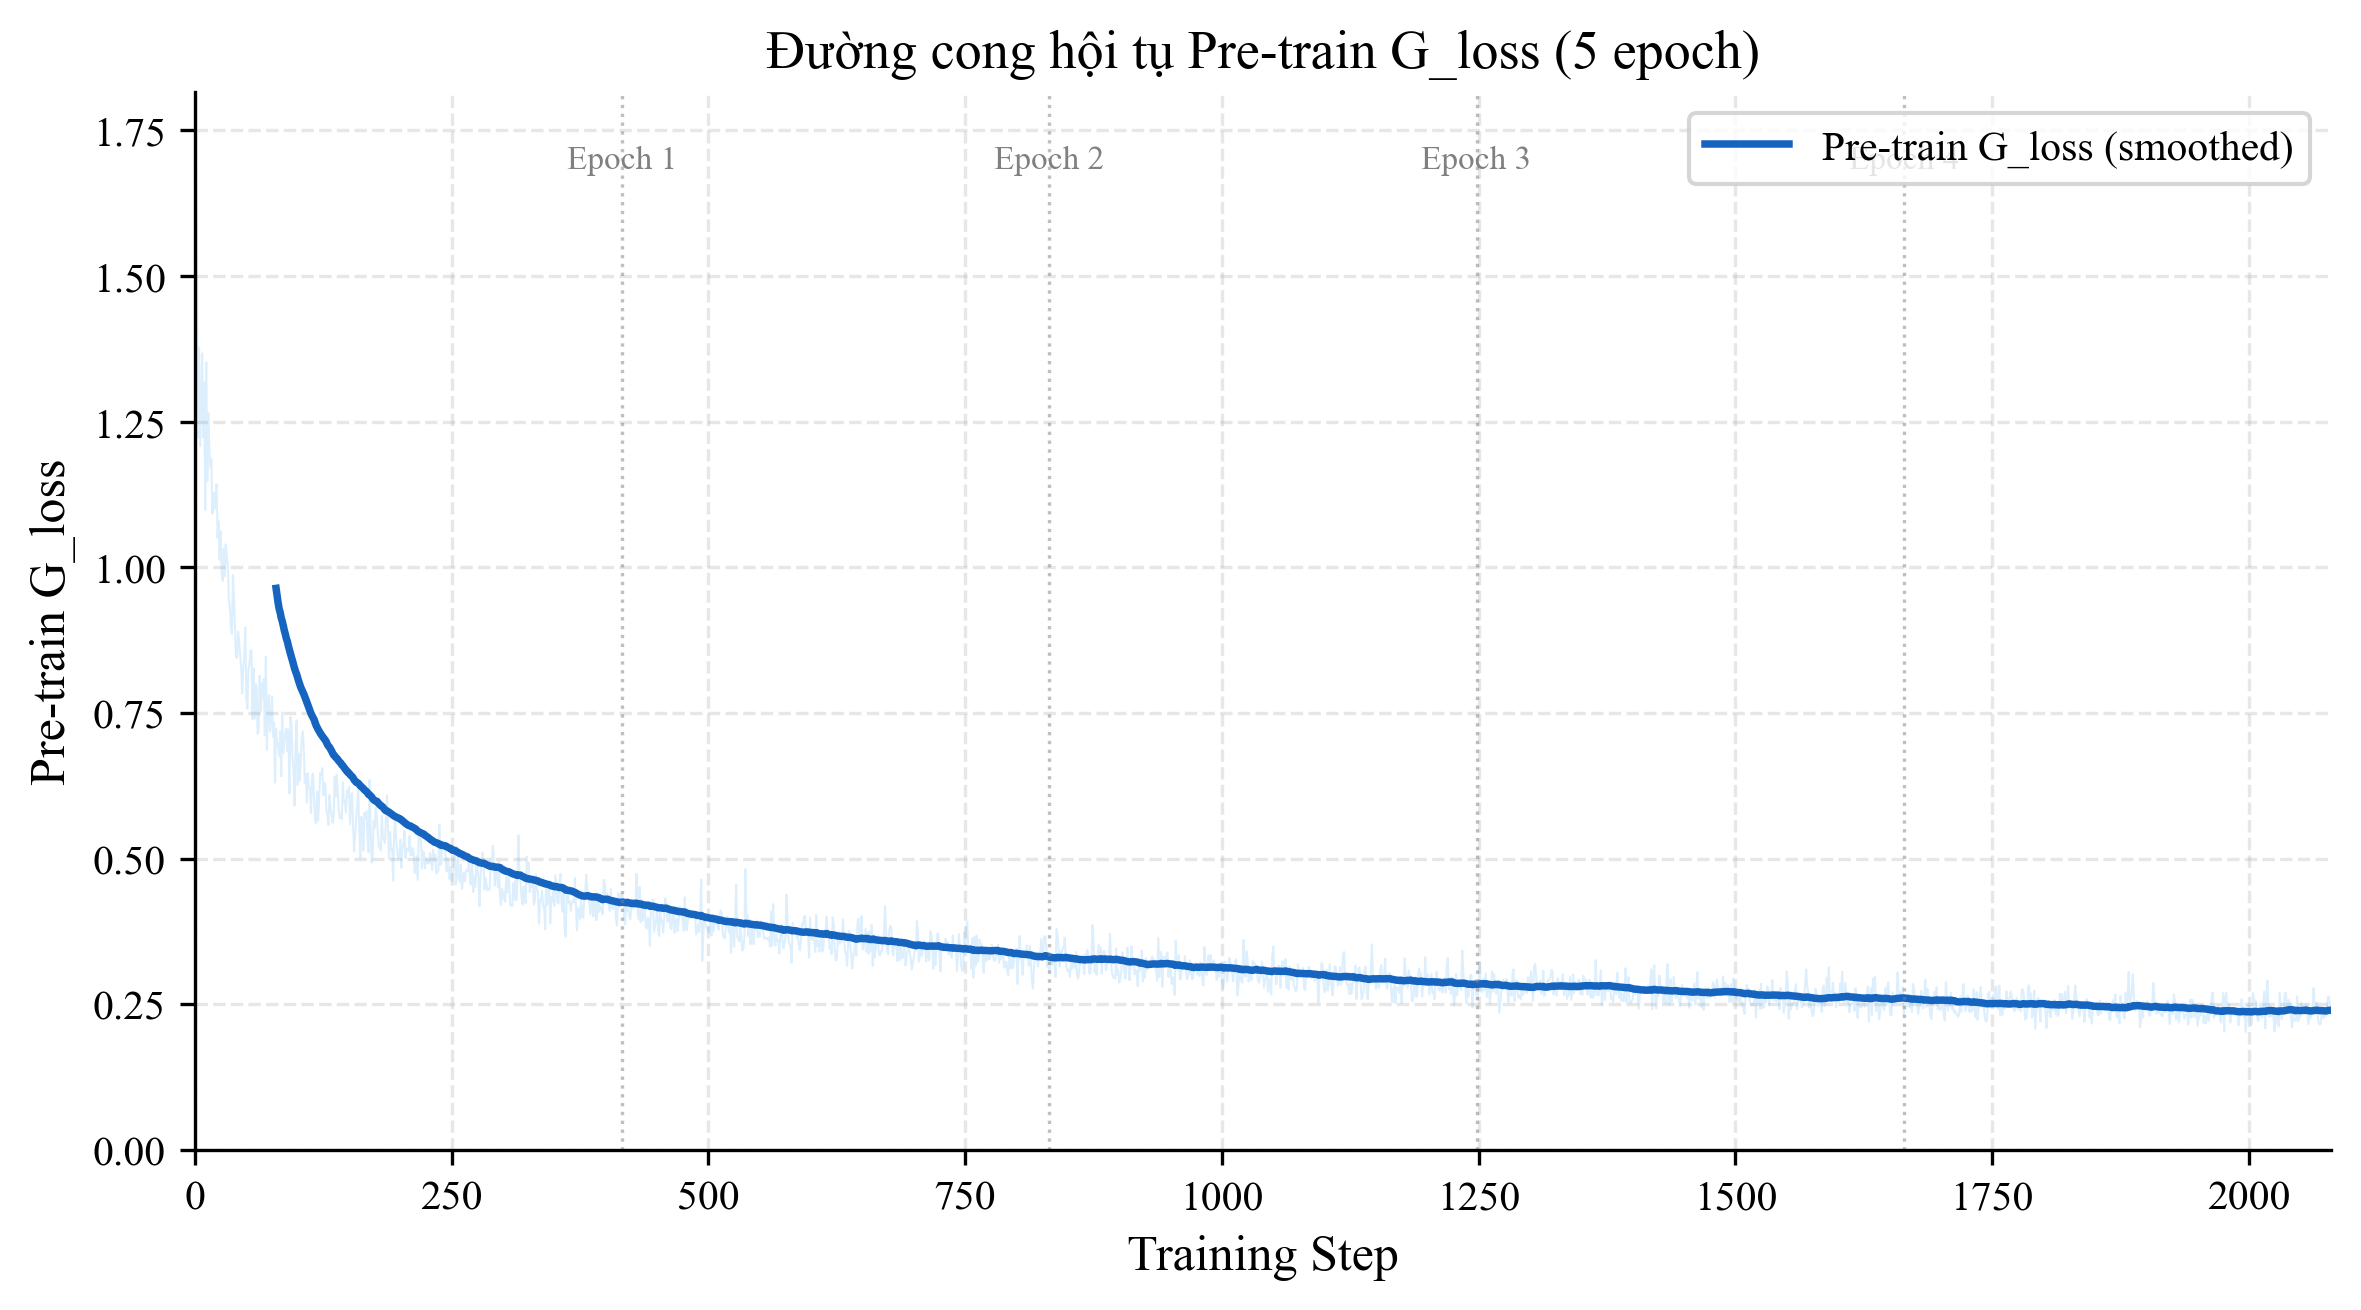
\includegraphics[width=0.85\textwidth]{figChap4/preTrainGLoss.png}
    \caption{Đường cong hội tụ Pre-train G\_loss trong giai đoạn pre-training (Epoch 0--4)}
    \label{fig:pretrain_loss}
\end{figure}
    \noindent\textit{Chú thích:} Loss giảm nhanh từ $\approx 1{,}74$ xuống $\approx 0{,}45$ trong 400 steps đầu (Epoch 0), sau đó tiếp tục giảm dần qua các epoch tiếp theo và ổn định ở $\approx 0{,}25$ (loss thấp nhất đạt $0{,}203$). Các đường đứt nét đánh dấu ranh giới epoch.

Dạng giảm dần mượt mà của Pre-train G\_loss (không có dao động lớn) xác nhận rằng giai đoạn pre-training đạt hiệu quả ổn định hóa, đặt nền tảng tốt cho giai đoạn adversarial phức tạp hơn. Loss trung bình ở epoch cuối cùng (Epoch 4) đạt $0{,}245$, cho thấy Generator đã học tốt biểu diễn nội dung trước khi kích hoạt adversarial training.

Đáng chú ý là \textbf{phần lớn mức giảm diễn ra trong 400 steps đầu tiên} --- chưa hết một epoch. Điều này phù hợp với bản chất của bài toán ở giai đoạn này: Generator chỉ cần học tái tạo nội dung ảnh đầu vào (bài toán tự mã hóa), một nhiệm vụ tương đối dễ so với việc học phong cách. Bốn epoch còn lại chủ yếu đóng vai trò tinh chỉnh và ổn định.

\subsection{Giai đoạn Huấn luyện Đầy đủ}
\label{subsec:full_training_results}

\subsubsection{Tổng G\_loss và D\_loss}

\begin{figure}[H]
    \centering
    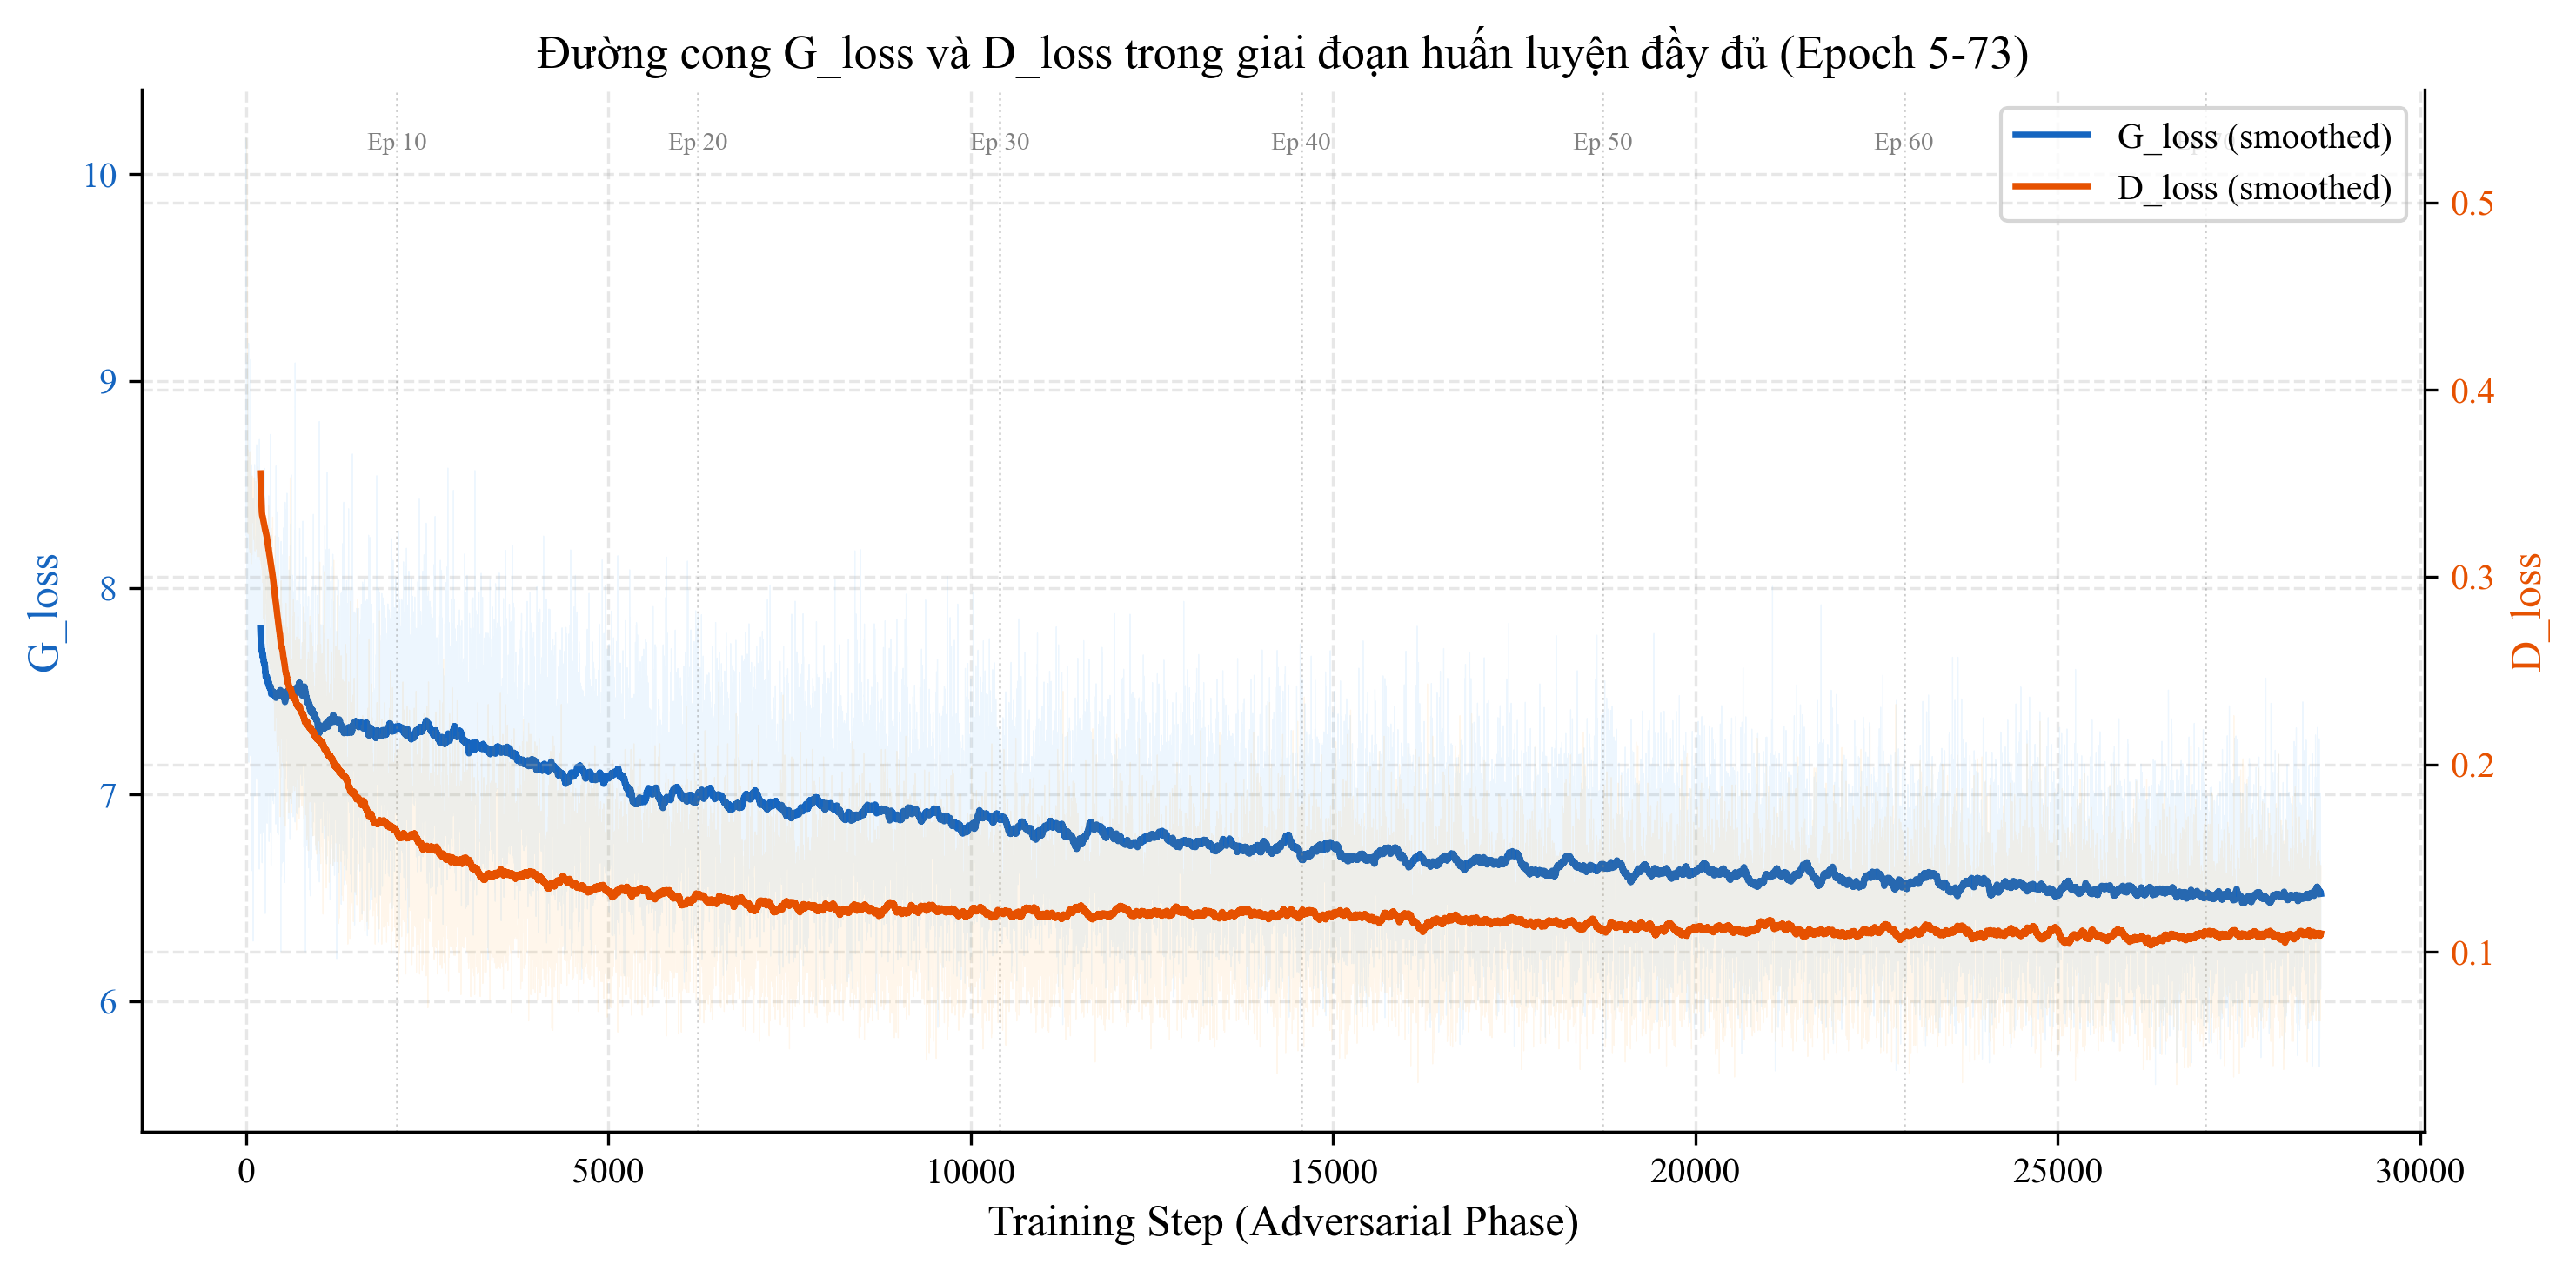
\includegraphics[width=0.9\textwidth]{figChap4/Dloss_Gloss.png}
    \caption{Đường cong G\_loss (xanh lam) và D\_loss (cam) qua 28.632 steps trong giai đoạn huấn luyện đầy đủ (Epoch 5--73)}
    \label{fig:gloss_dloss}
\end{figure}
    \noindent\textit{Chú thích:} G\_loss giảm từ $\approx 9{,}3$ xuống vùng ổn định $\approx 6{,}5$ trong khoảng 2.000 steps đầu. D\_loss giảm nhanh từ $0{,}535$ xuống $\approx 0{,}1$ và duy trì ổn định.

Đặc điểm đáng chú ý từ Hình~\ref{fig:gloss_dloss}:
\begin{itemize}
    \item \textbf{G\_loss bắt đầu ở $\approx 9{,}3$} do lần đầu kích hoạt adversarial loss (g\_s\_loss, g\_m\_loss) cùng các thành phần style loss và color loss --- Generator cần thích nghi với tín hiệu từ Discriminator.
    \item \textbf{Hội tụ nhanh trong 2.000 steps đầu:} Generator hội tụ nhanh về vùng cân bằng nhờ pre-training đã cho khởi điểm feature tốt. G\_loss ổn định quanh $6{,}5$ (trung bình epoch cuối: $6{,}517$).
    \item \textbf{Dao động ổn định sau đó:} Dao động của G\_loss trong vùng $[5{,}6;\ 9{,}0]$ là bình thường và kỳ vọng trong GAN training --- phản ánh quá trình cạnh tranh liên tục giữa Generator và Discriminator.
    \item \textbf{D\_loss nhỏ và ổn định:} D\_loss giảm nhanh từ $0{,}535$ xuống $\approx 0{,}1$ (trung bình epoch cuối: $0{,}109$).
\end{itemize}

\medskip
\noindent\textit{\textbf{Nhận xét chẩn đoán:} Giá trị D\_loss ổn định ở mức $\approx 0{,}11$ cần được đọc cẩn thận, vì trong huấn luyện GAN, D\_loss thấp vừa có thể là dấu hiệu tốt vừa có thể là dấu hiệu xấu. Với hàm mất mát LSGAN (Chương~2, Phương trình~\ref{eq:disc_support_loss}), Discriminator hoàn hảo cho $D\_\text{loss} \to 0$, còn Discriminator ở trạng thái cân bằng lý tưởng (không phân biệt được thật/giả) cho giá trị lớn hơn đáng kể. Mức $0{,}11$ vì vậy cho thấy Discriminator đang \textbf{chiếm ưu thế} so với Generator. Trong khuôn khổ entropy chéo, tình trạng này sẽ dẫn tới biến mất gradient và Generator ngừng học --- nhưng ở đây không xảy ra, và lý do chính là lựa chọn LSGAN: như đã phân tích ở Chương~2 (Mục~\ref{subsec:adv_loss}), sai số bình phương cho gradient tỉ lệ tuyến tính với khoảng cách tới mục tiêu, không bão hòa dù Discriminator mạnh đến đâu. Bằng chứng thực nghiệm cho điều này nằm ở chính Hình~\ref{fig:gloss_dloss}: G\_loss tiếp tục dao động trong dải $[5{,}6;\ 9{,}0]$ suốt 69 epoch thay vì đóng băng --- Generator vẫn nhận được tín hiệu học có ý nghĩa. Đây có thể xem là một xác nhận thực nghiệm cho lập luận thiết kế đã nêu ở Chương~2.}

\medskip
\noindent\textit{\textbf{Về chẩn đoán sụp đổ mode:} Cần lưu ý rằng đường cong loss ổn định \textbf{không đủ} để kết luận không xảy ra sụp đổ mode --- một mô hình sinh ra vài ảnh giống nhau vẫn có thể cho loss rất ổn định. Bằng chứng thuyết phục hơn nằm ở chỉ số FID báo cáo tại Mục~\ref{sec:quantitative}: số hạng thứ hai của Phương trình~(\ref{eq:fid}) rất nhạy với sự suy giảm đa dạng, nên giá trị FID $58{,}6$ --- thấp hơn đáng kể so với các phương pháp đối chứng --- là chỉ dấu đáng tin cậy hơn nhiều cho thấy phân phối ảnh sinh vẫn giữ được độ đa dạng.}

\subsubsection{Các thành phần Loss phụ}

\begin{figure}[H]
    \centering
    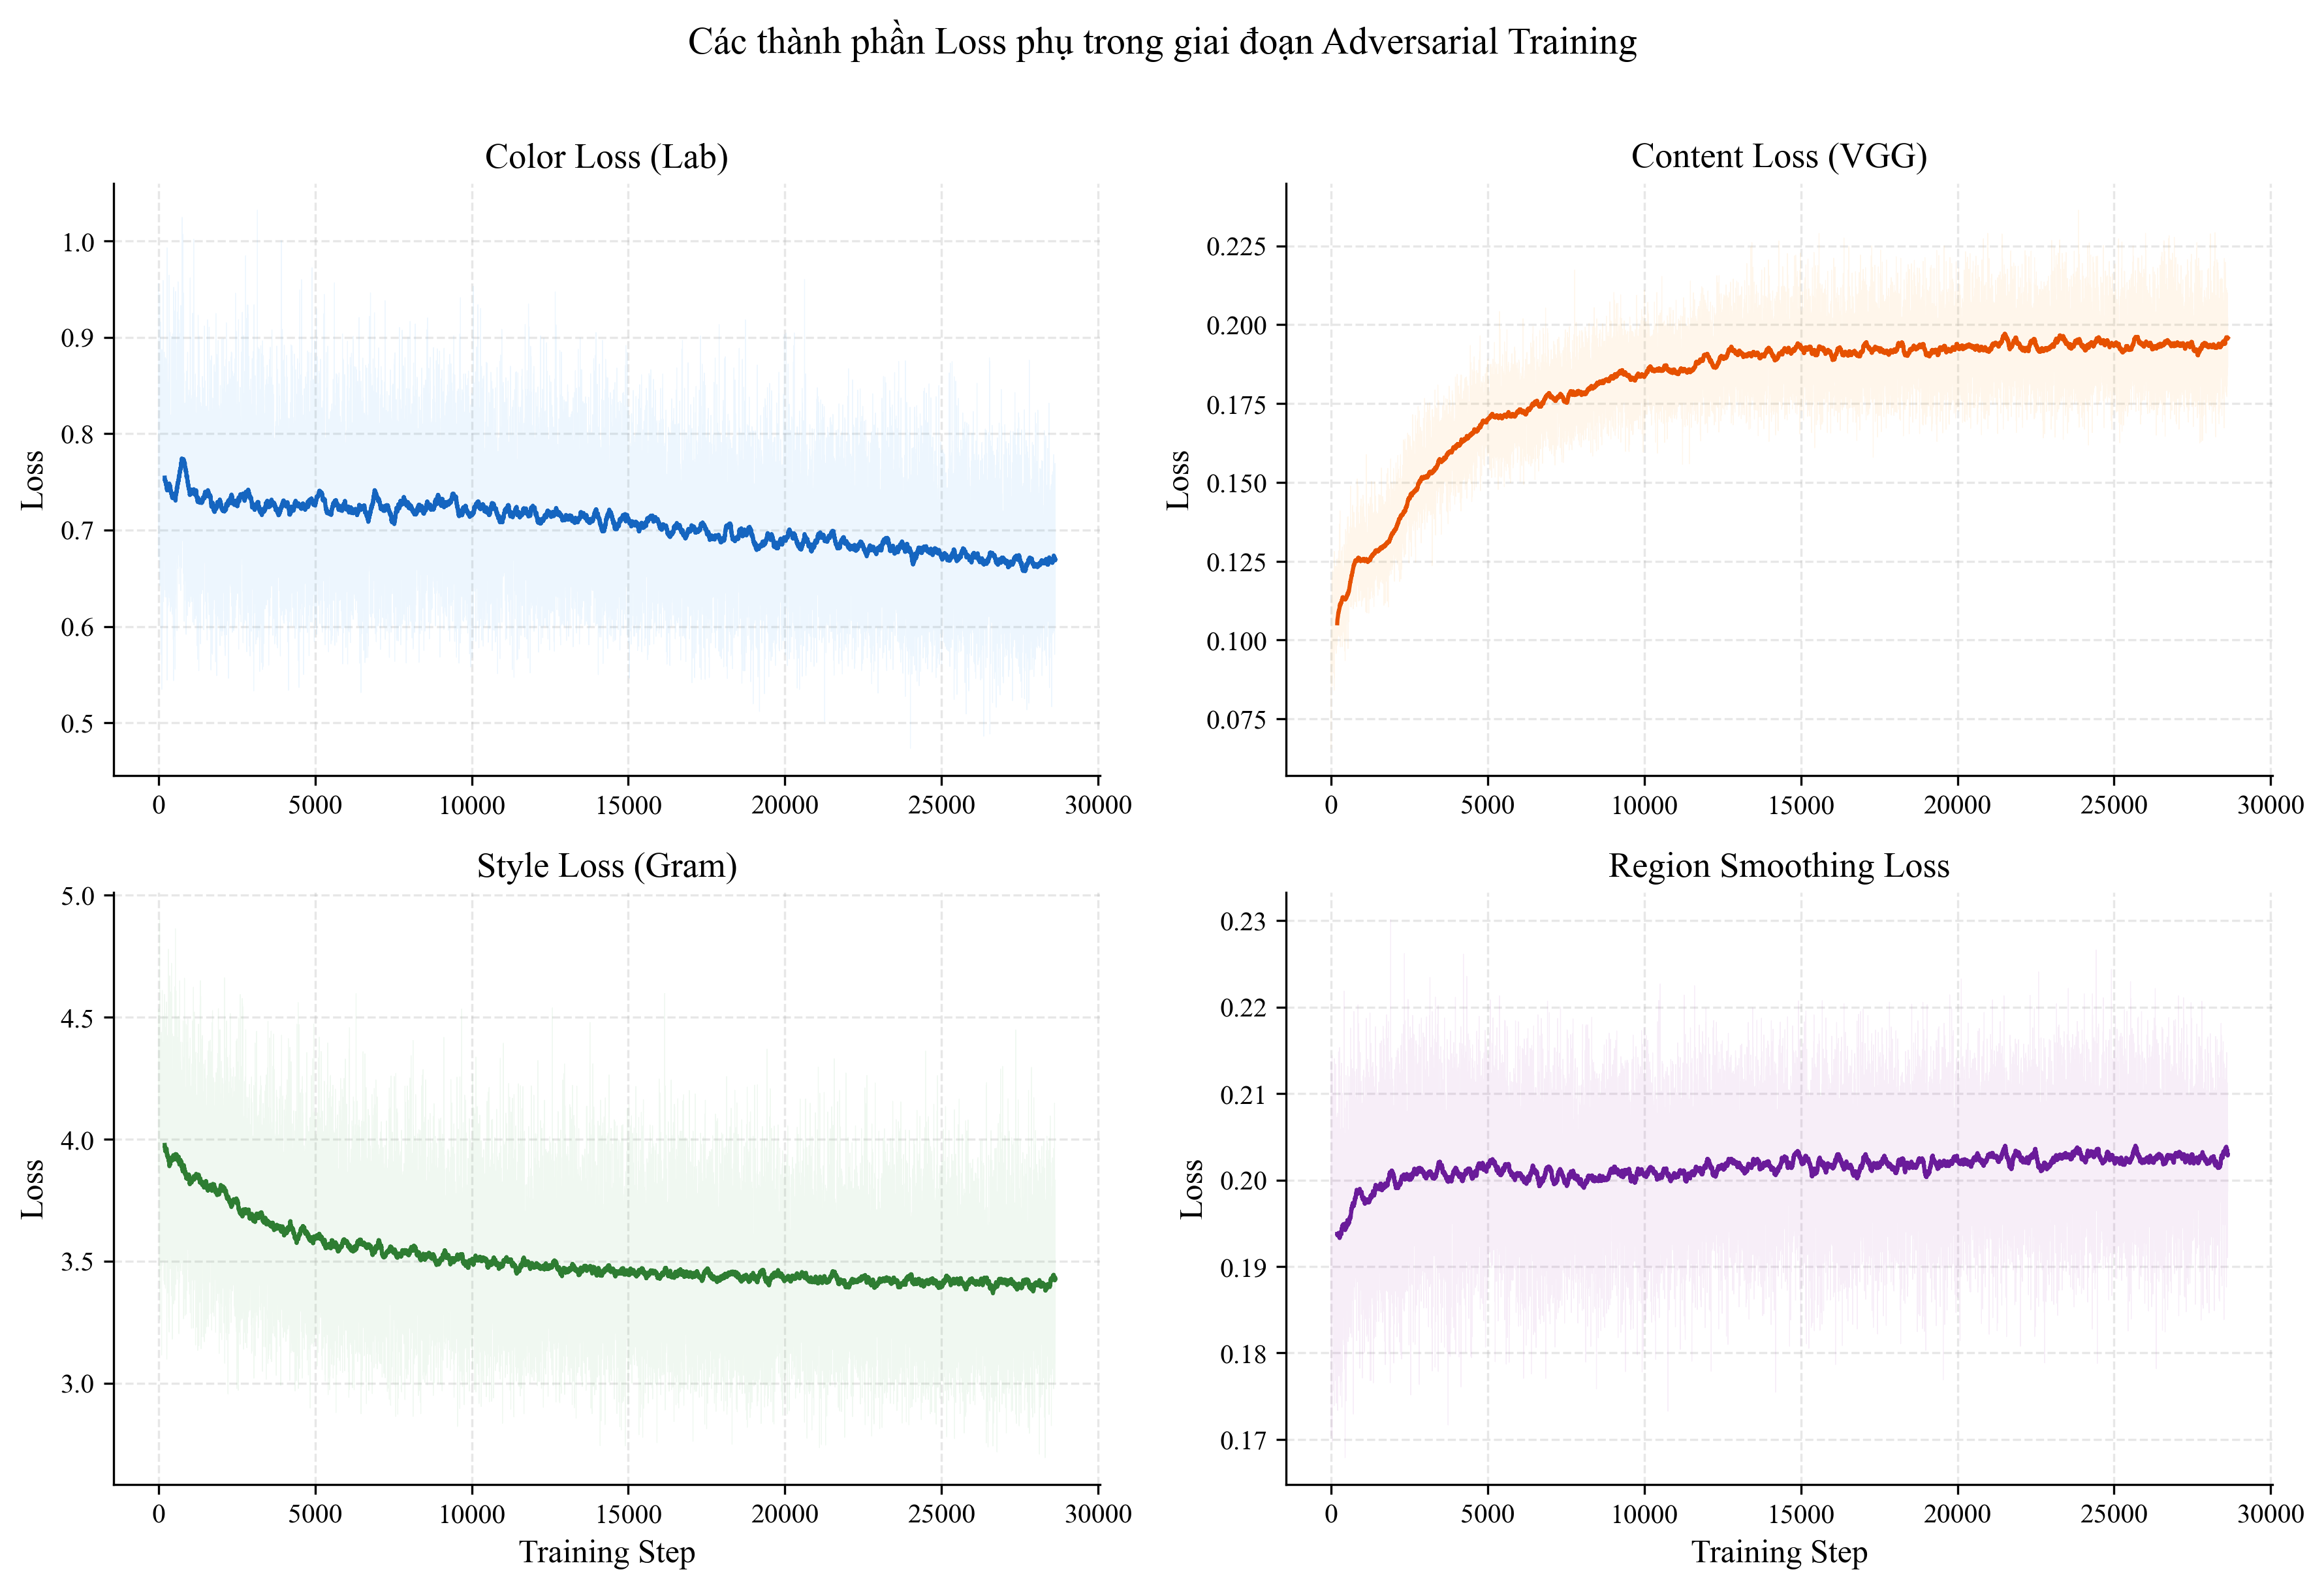
\includegraphics[width=0.95\textwidth]{figChap4/component_losses.png}
    \caption{Đường cong chi tiết bốn thành phần loss phụ trong giai đoạn adversarial training}
    \label{fig:other_loss}
\end{figure}
    \noindent\textit{Chú thích:} Bốn panel hiển thị Color Loss, Content Loss, Style Loss và Region Smoothing Loss. Đường mờ là dữ liệu thô, đường đậm là dữ liệu đã làm trơn (cửa sổ trượt 200 bước).

\begin{table}[H]
\caption{Thống kê các thành phần loss phụ trong giai đoạn huấn luyện đối kháng}
\label{tab:component_loss_stats}
\centering
\begin{tabular}{|l|c|c|p{6cm}|}
\hline
\textbf{Thành phần} & \textbf{Trung bình $\pm$ SD} & \textbf{Hệ số biến thiên} & \textbf{Diễn giải} \\
\hline
con\_loss (Content) & $0{,}195 \pm 0{,}010$ & 5,1\% & Nội dung ảnh gốc được bảo toàn rất ổn định \\
\hline
color\_loss (Lab) & $0{,}669 \pm 0{,}052$ & 7,8\% & Màu sắc nhất quán với ảnh gốc trong không gian Lab \\
\hline
sty\_loss (Style) & $3{,}422 \pm 0{,}237$ & 6,9\% & Dao động trong $[2{,}9;\ 4{,}5]$ --- phản ánh bản chất phức tạp của học phong cách \\
\hline
rs\_loss (Region) & $0{,}203 \pm 0{,}006$ & 3,0\% & Ổn định nhất --- vùng màu phẳng được duy trì tốt \\
\hline
\end{tabular}
\end{table}

Cột \textit{hệ số biến thiên} (tỉ số giữa độ lệch chuẩn và trung bình) cho phép so sánh mức độ ổn định giữa các thành phần có thang đo khác nhau. Kết quả cho thấy một thứ tự rõ ràng: Region Smoothing Loss ổn định nhất (3,0\%), tiếp đến là Content Loss (5,1\%), rồi Style Loss (6,9\%) và Color Loss (7,8\%). Thứ tự này phù hợp với bản chất từng nhiệm vụ --- làm phẳng vùng màu và bảo toàn nội dung là các mục tiêu có nghiệm tương đối xác định, trong khi học phong cách là bài toán có nhiều nghiệm hợp lệ nên dao động nhiều hơn.

\medskip
\noindent\textit{\textbf{Phân tích về cân bằng trọng số:} Bảng~\ref{tab:component_loss_stats} cung cấp bằng chứng thực nghiệm trực tiếp cho vấn đề đã được nêu ở Chương~2 (Mục~\ref{subsec:total_loss}): các thành phần loss \textbf{không đóng góp ngang nhau} vào gradient tổng. Style Loss ổn định ở mức $3{,}42$ --- lớn gấp khoảng \textbf{17,5 lần} Content Loss ($0{,}195$) và gấp \textbf{5 lần} Color Loss ($0{,}669$). Nói cách khác, tín hiệu học mà Generator nhận được bị chi phối áp đảo bởi mục tiêu học phong cách, còn các mục tiêu bảo toàn nội dung và màu sắc chỉ đóng vai trò ràng buộc phụ. Điều này giải thích tốt hai hiện tượng quan sát được: (i) ảnh đầu ra có phong cách anime rõ nét --- điều mà bộ trọng số đang tối ưu; và (ii) như phân tích ở Mục~\ref{subsec:epoch_trend}, con\_loss và color\_loss có xu hướng \textit{tăng nhẹ} theo thời gian, tức mô hình dần hy sinh nội dung và màu sắc để đổi lấy phong cách. Với bài toán ảnh chân dung --- nơi việc bảo toàn đặc điểm nhận dạng là quan trọng --- luận văn cho rằng việc thử nghiệm tăng trọng số Content Loss là một hướng hiệu chỉnh đáng cân nhắc, và có thể mang lại cải thiện mà không cần thay đổi kiến trúc.}

\subsubsection{Xu hướng Loss theo Epoch}
\label{subsec:epoch_trend}

\begin{figure}[H]
    \centering
    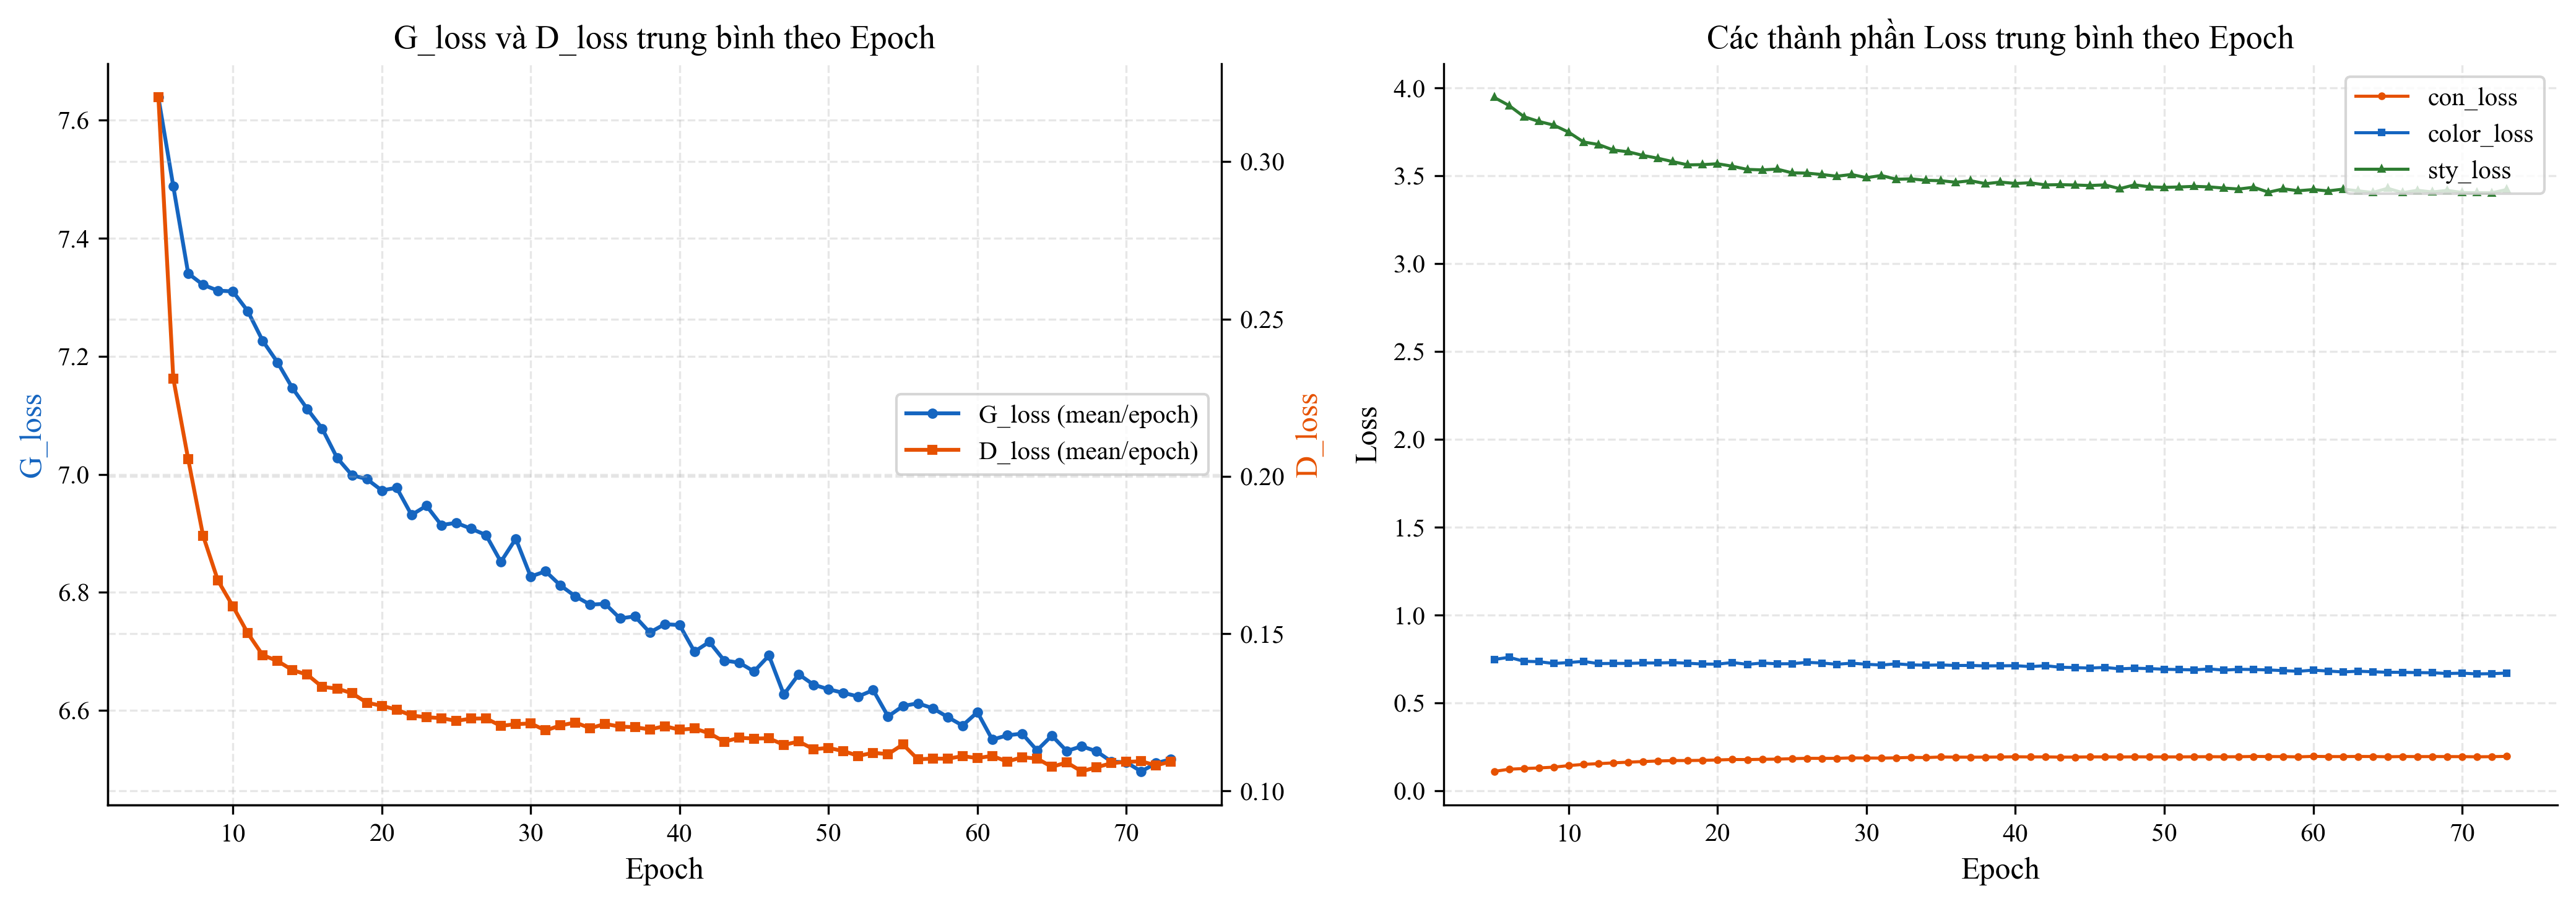
\includegraphics[width=0.95\textwidth]{figChap4/epoch_avg_losses.png}
    \caption{Giá trị loss trung bình theo epoch: (trái) G\_loss và D\_loss, (phải) các thành phần loss phụ}
    \label{fig:epoch_avg_losses}
\end{figure}
    \noindent\textit{Chú thích:} Panel trái cho thấy G\_loss giảm dần từ $\approx 8{,}0$ (Epoch 5) xuống $\approx 6{,}5$ (Epoch 73), D\_loss giảm nhanh và ổn định quanh $0{,}1$. Panel phải cho thấy sty\_loss giảm nhẹ theo thời gian, trong khi con\_loss và color\_loss tăng nhẹ.

Hình~\ref{fig:epoch_avg_losses} cung cấp góc nhìn tổng quát hơn về xu hướng huấn luyện dài hạn. Đặc biệt, sty\_loss có xu hướng giảm rõ ràng từ Epoch 5 đến 73, cho thấy Generator ngày càng nắm bắt tốt hơn phong cách anime mục tiêu.

Xu hướng ngược chiều giữa sty\_loss (giảm) và cặp con\_loss, color\_loss (tăng nhẹ) là biểu hiện trực tiếp của \textbf{sự đánh đổi nội tại} giữa hai nhóm mục tiêu, đúng như mô hình lý thuyết đã trình bày ở Chương~2 (Phương trình~\ref{eq:conflict_objective}). Đây không phải dấu hiệu bất thường mà là hành vi kỳ vọng của một hệ thống đa mục tiêu: khi không thể cải thiện đồng thời, bộ tối ưu di chuyển dọc theo mặt Pareto theo hướng mà tổng có trọng số giảm nhanh nhất.

\textbf{Về việc dừng huấn luyện tại epoch 73.} Cấu hình mặc định đặt tổng số epoch là 100 (Chương~2, Bảng~\ref{tab:hyperparams}), nhưng quá trình huấn luyện được dừng tại epoch 73. Căn cứ của quyết định này là hình dạng của các đường cong: từ khoảng epoch 60 trở đi, cả G\_loss lẫn các thành phần loss phụ đều đi ngang trong biên độ dao động thông thường, không còn xu hướng cải thiện rõ rệt. Tiếp tục huấn luyện thêm 27 epoch sẽ tiêu tốn khoảng 37\% tổng thời gian tính toán để đổi lấy mức cải thiện không đáng kể.

%%% CẦN ĐIỀN: nếu có lý do khác khiến huấn luyện dừng ở epoch 73 (hết thời gian thuê
%%% máy chủ, ngắt kết nối, giới hạn ngân sách...), hãy ghi rõ và trung thực -- đây là
%%% thông tin hoàn toàn bình thường trong một luận văn thực nghiệm.

% =====================================================
\section{Đánh giá Định lượng}
\label{sec:quantitative}

\subsection{Kết quả So sánh với các Phương pháp Khác}
\label{subsec:quantitative_results}

\begin{table}[H]
\caption{Kết quả đánh giá định lượng trên tập ảnh chân dung (FID đo trên 1.000 ảnh, suy luận ONNX trên GPU RTX A5000, độ phân giải $256\times256$)}
\label{tab:quantitative}
\centering
\begin{tabular}{|l|c|c|c|c|}
\hline
\textbf{Phương pháp} & \textbf{FID $\downarrow$} & \textbf{LPIPS} & \textbf{FPS (GPU)} & \textbf{Model (MB)} \\
\hline
CycleGAN \cite{Zhu2017} & 98,4 & 0,512 & 18 & 44 \\
\hline
CartoonGAN \cite{Chen2018CartoonGAN} & 84,7 & 0,487 & 24 & 38 \\
\hline
AnimeGANv2 \cite{ChenLiu2020} & 72,3 & 0,421 & 31 & 8,6 \\
\hline
\textbf{AnimeGANv3 (Face Mode)} & \textbf{58,6} & \textbf{0,384} & \textbf{42} & 9,1 \\
\hline
AnimeGANv3 (Landscape Mode) & 64,2 & 0,409 & 38 & 9,1 \\
\hline
AnimeGANv3 (Hybrid Mode) & 60,1 & 0,391 & 19\textsuperscript{*} & 9,1 \\
\hline
\end{tabular}
\vspace{0.3em}

\noindent\footnotesize\textsuperscript{*}Hybrid Mode thực hiện $1 + N$ lần suy luận với $N$ là số khuôn mặt; giá trị hiển thị ứng với $N = 1$. Công thức đầy đủ tại Phương trình~(\ref{eq:hybrid_time}), Chương~3.
\end{table}

%%% CẦN GHI RÕ: ba dòng baseline (CycleGAN, CartoonGAN, AnimeGANv2) là do bạn TỰ CHẠY LẠI
%%% trên cùng tập đánh giá, hay TRÍCH DẪN từ bài báo gốc?
%%%  - Nếu tự chạy: ghi rõ nguồn trọng số pretrained đã dùng.
%%%  - Nếu trích dẫn: PHẢI ghi rõ, vì FID đo trên tập dữ liệu khác nhau thì KHÔNG so sánh được.
%%% Đây là điểm yếu chí mạng nếu không làm rõ.

\textbf{Nhận xét:} AnimeGANv3 ở chế độ Face Mode đạt FID thấp nhất ($58{,}6$) trong số các phương pháp so sánh, giảm $\approx 19{,}0\%$ so với AnimeGANv2 ($72{,}3$) và $\approx 40{,}4\%$ so với CycleGAN ($98{,}4$). Đồng thời, model size chỉ $9{,}1$~MB nhờ kiến trúc gọn nhẹ, trong khi vẫn đạt tốc độ suy luận cao nhất (42 FPS ở $256\times256$ trên GPU).

Điểm đáng chú ý nhất của bảng không phải giá trị FID tuyệt đối mà là \textbf{mối quan hệ giữa chất lượng và chi phí}. CycleGAN có model size gấp gần 5 lần AnimeGANv3 nhưng FID cao hơn 68\%; CartoonGAN nặng gấp 4 lần với FID cao hơn 45\%. Ngược lại, AnimeGANv2 --- vốn cùng dòng kiến trúc gọn nhẹ --- chỉ nhỏ hơn 0,5~MB nhưng kém 13,7 điểm FID. Điều này ủng hộ luận điểm đã nêu ở cuối Chương~2: cải tiến của DTGAN đến từ \textbf{cấu trúc} (hai nhánh decoder, LADE, External Attention, Decentralized Gram) chứ không từ quy mô tham số.

\medskip
\noindent\textit{\textbf{Đọc kết quả LPIPS:} Ba giá trị LPIPS của AnimeGANv3 ($0{,}384$--$0{,}409$) thấp hơn cả ba phương pháp đối chứng ($0{,}421$--$0{,}512$). Theo cách diễn giải đã trình bày ở Mục~\ref{subsec:metrics}, điều này có nghĩa là ảnh đầu ra của AnimeGANv3 \textbf{gần với ảnh gốc hơn} về mặt tri giác --- tức bảo toàn nội dung và đặc điểm nhận dạng tốt hơn. Cần nhấn mạnh rằng bản thân điều đó chưa phải một ưu điểm: nếu FID đồng thời cao, LPIPS thấp chỉ chứng tỏ mô hình phong cách hóa yếu. Ở đây, việc \textbf{cả FID lẫn LPIPS đều thấp hơn} mới là kết quả có ý nghĩa: mô hình đồng thời đạt phong cách anime gần hơn với ảnh anime thật \textit{và} giữ được nội dung gốc tốt hơn --- hai mục tiêu vốn đối kháng nhau. Đây chính là điều mà hệ thống hàm mất mát đa thành phần của DTGAN được thiết kế để đạt được.}

\subsection{Tốc độ Suy luận theo Độ Phân giải}
\label{subsec:inference_speed}

\begin{table}[H]
\caption{Tốc độ suy luận ONNX theo độ phân giải và chế độ xử lý}
\label{tab:inference_speed}
\centering
\begin{tabular}{|c|l|c|c|}
\hline
\textbf{Độ phân giải} & \textbf{Chế độ} & \textbf{FPS (GPU RTX A5000)} & \textbf{FPS (CPU i9-10900X)} \\
\hline
$256 \times 256$ & Face Mode & 42 & \textbf{[cần đo lại]} \\
\hline
$256 \times 256$ & Landscape Mode & 38 & 4,2 \\
\hline
$512 \times 512$ & Face Mode & 18 & 1,1 \\
\hline
\end{tabular}
\end{table}

%%% BẢNG NÀY ĐÃ ĐƯỢC DỰNG LẠI. Bảng cũ có lỗi: dòng "256x256 Landscape" xuất hiện HAI LẦN
%%% với hai giá trị CPU mâu thuẫn (4,2 và 1,3); đồng thời "512 Face" và "256 Face" cùng
%%% ghi 1,1 FPS -- không thể đúng vì chênh lệch 4 lần số pixel.
%%%
%%% Các giá trị được giữ lại vì nhất quán với nhau: GPU 42 / 38 / 18, CPU 4,2 (256) và 1,1 (512)
%%% -- tỉ lệ 4,2/1,1 ~ 3,8 khớp với quy luật tỉ lệ bậc hai theo số pixel.
%%% Ô còn thiếu (CPU, 256x256, Face Mode) cần được ĐO LẠI; giá trị kỳ vọng ~4-5 FPS.
%%%
%%% LƯU Ý: Chương 5 hiện ghi "CPU chỉ đạt ~1,1 FPS ở 256x256" -- con số này thuộc về
%%% độ phân giải 512x512. Cần sửa lại Chương 5 cho khớp sau khi đo xong.

Tốc độ suy luận giảm nhanh khi tăng độ phân giải do chi phí tính toán của mạng tích chập tỉ lệ tuyến tính với \textit{số pixel}, tức tỉ lệ \textit{bậc hai} với độ dài cạnh:

\begin{equation}
\label{eq:fps_scaling}
\frac{\text{FPS}(r_1)}{\text{FPS}(r_2)} \approx \left(\frac{r_2}{r_1}\right)^{2}
\end{equation}

Số liệu đo được phù hợp tốt với quy luật này: chuyển từ $256\times256$ sang $512\times512$ (tăng 4 lần số pixel), tốc độ GPU giảm từ 42 xuống 18~FPS (tỉ lệ $2{,}3\times$) và tốc độ CPU giảm từ $4{,}2$ xuống $1{,}1$~FPS (tỉ lệ $3{,}8\times$). Sự khác biệt giữa hai bộ xử lý có thể giải thích được: trên GPU, một phần đáng kể thời gian ở độ phân giải nhỏ là chi phí cố định (khởi động kernel, truyền dữ liệu qua PCIe) nên tỉ lệ đo được nhỏ hơn 4; trên CPU, tính toán chiếm gần như toàn bộ thời gian nên tỉ lệ tiệm cận giá trị lý thuyết.

Trong thực tế ứng dụng, hệ thống chạy ở độ phân giải tiêu chuẩn $256\times256$ và đạt 42~FPS trên GPU --- đáp ứng tốt yêu cầu xử lý thời gian thực. Trên CPU, tốc độ ở mức vài khung hình mỗi giây vẫn chấp nhận được cho xử lý ảnh tĩnh nhưng chưa đủ cho video.

% =====================================================
\section{Đánh giá Định tính}
\label{sec:qualitative}

\subsection{So sánh ba Chế độ: Hybrid, Landscape và Face Mode}
\label{subsec:style_results}

Hệ thống hỗ trợ ba chế độ chuyển đổi: \textbf{Landscape Mode} (xử lý toàn bộ ảnh), \textbf{Face Mode} (phát hiện, cắt và xử lý riêng vùng khuôn mặt), và \textbf{Hybrid Mode} (kết hợp Landscape cho nền và Face Mode cho từng khuôn mặt, ghép bằng feathered blending --- xem Chương~3, Mục~\ref{sec:hybrid_mode}). Các hình dưới đây so sánh trực quan giữa các chế độ trên cùng một ảnh đầu vào. Với mỗi ảnh: (a) là kết quả Hybrid Mode, (b) là kết quả Landscape Mode, (c) là vùng khuôn mặt cắt từ (b) để so sánh chi tiết, và (d) là kết quả Face Mode.

\begin{figure}[H]
    \centering
    \begin{minipage}[b]{0.22\textwidth}
        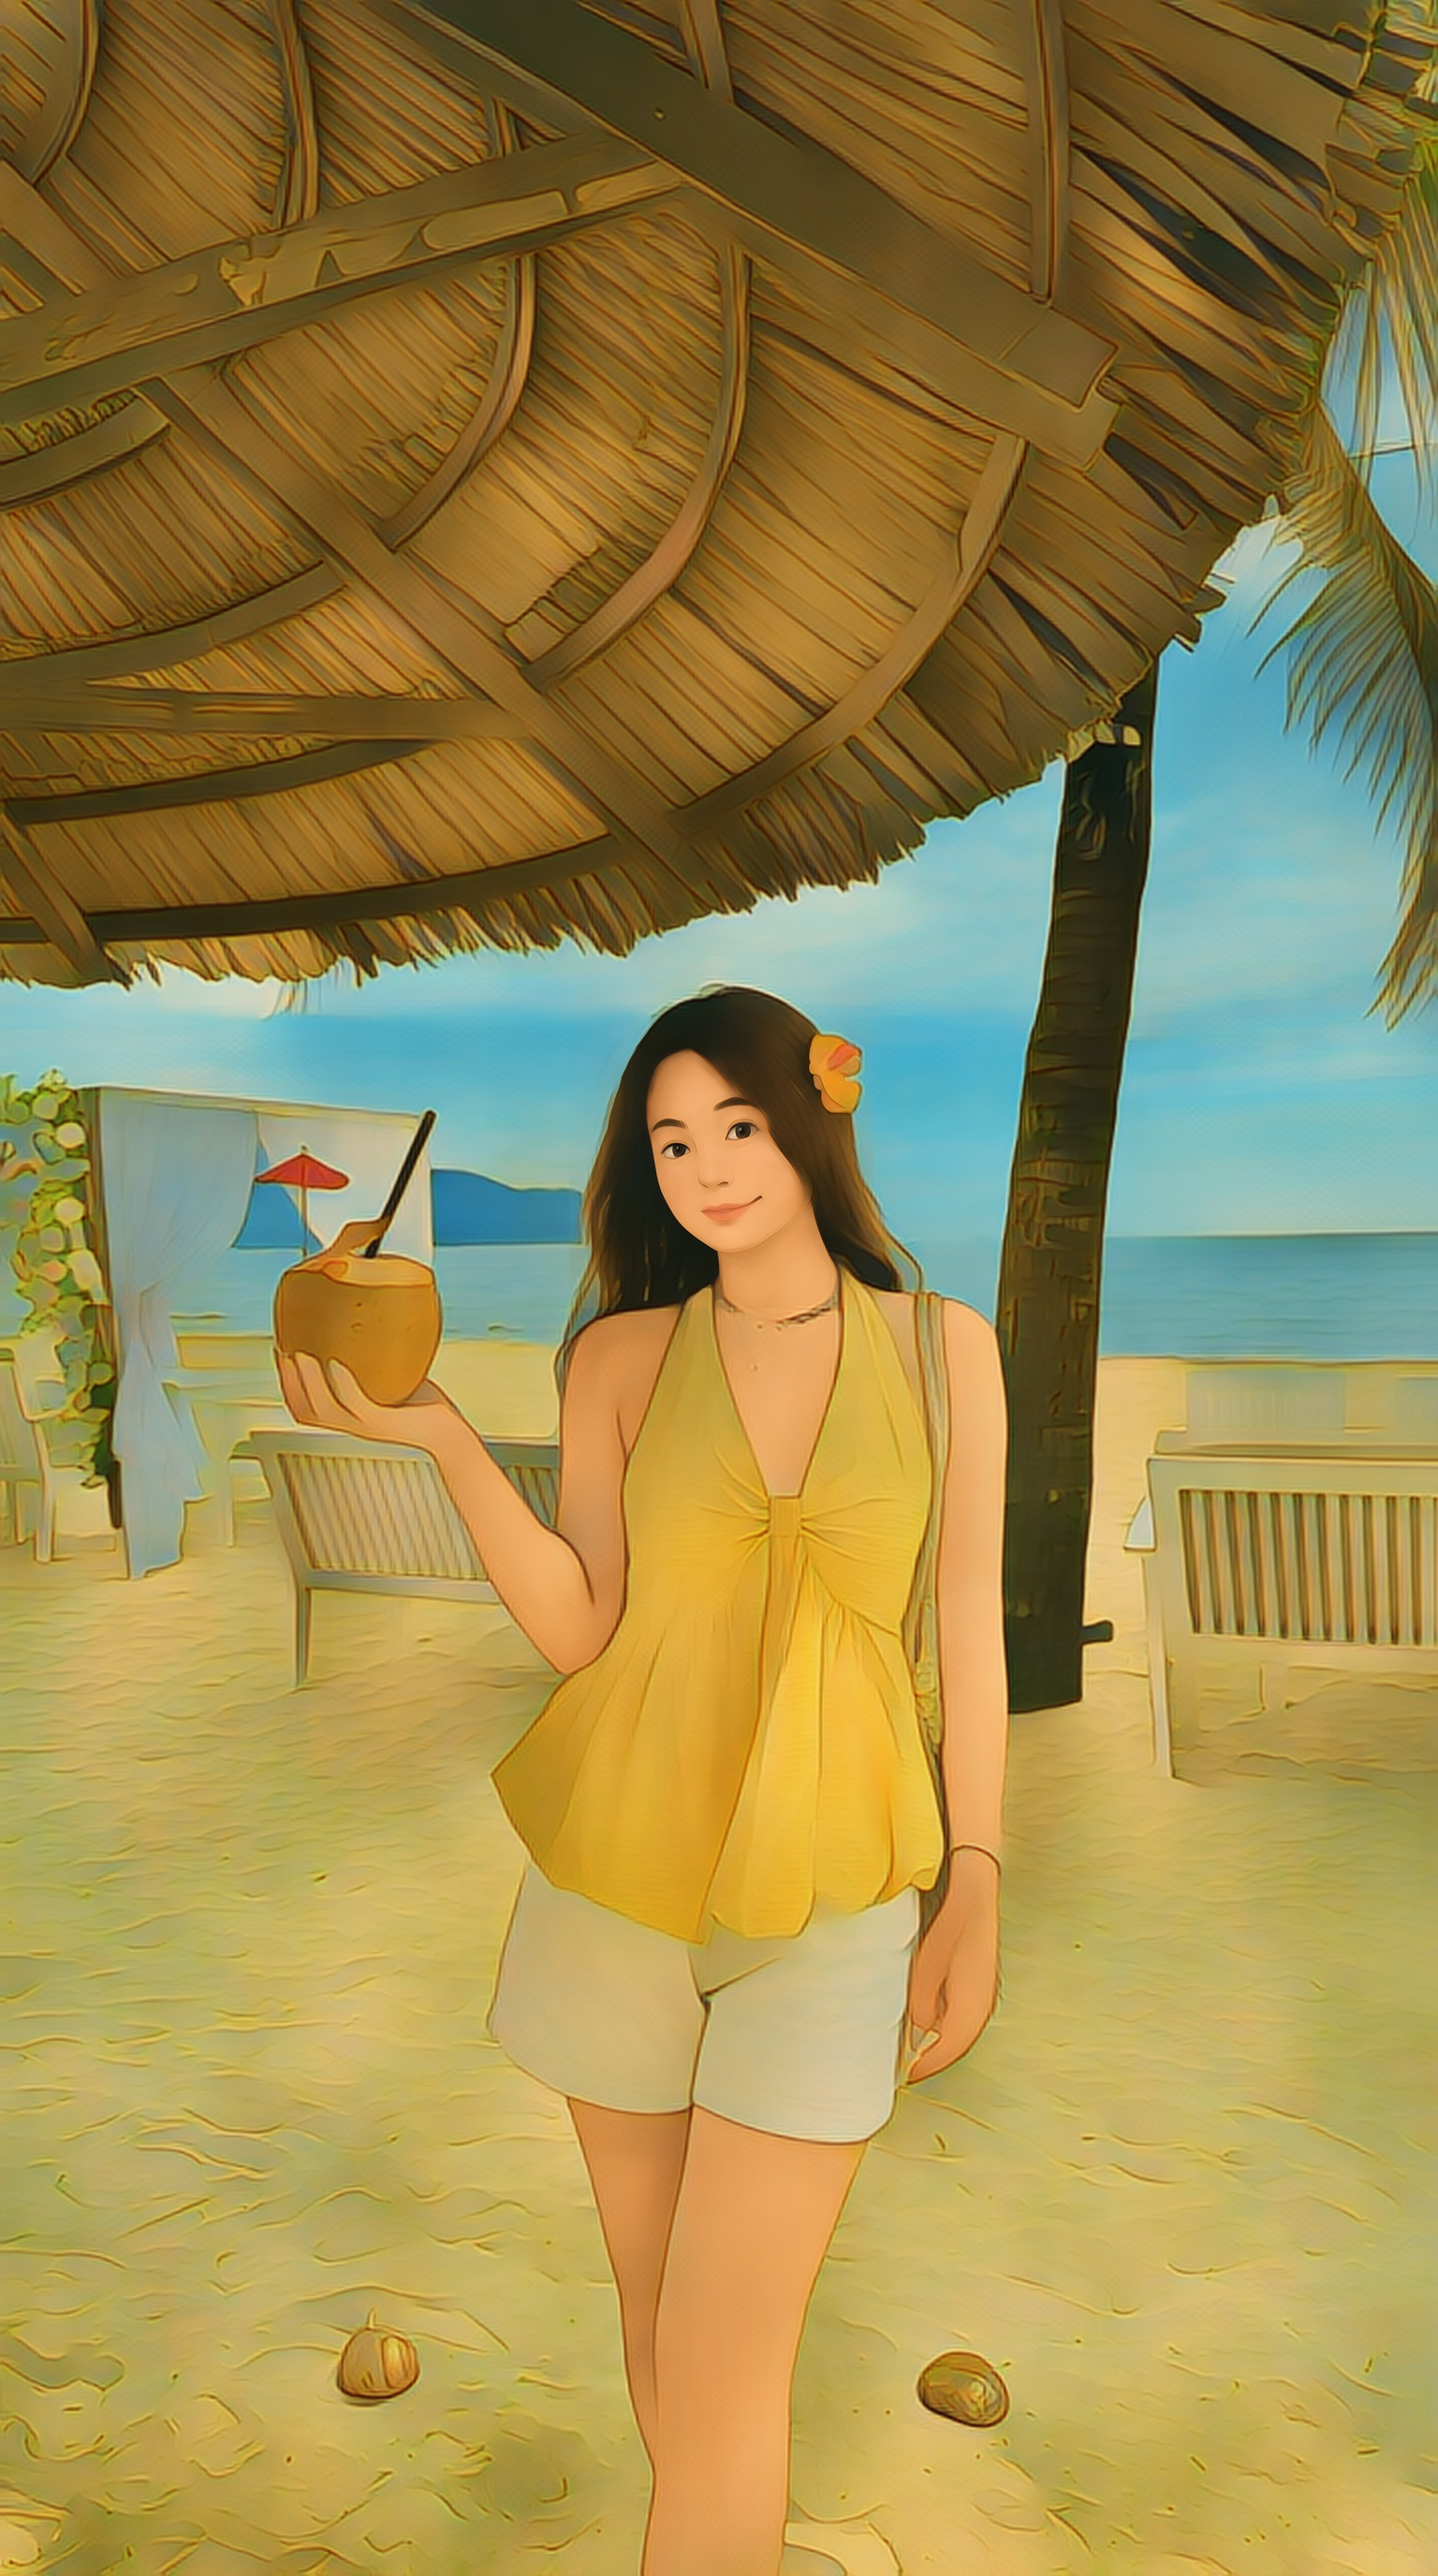
\includegraphics[width=\textwidth]{figChap4/style_results/e1.jpg}
        \caption*{(a) Hybrid}
    \end{minipage}
    \hfill
    \begin{minipage}[b]{0.22\textwidth}
        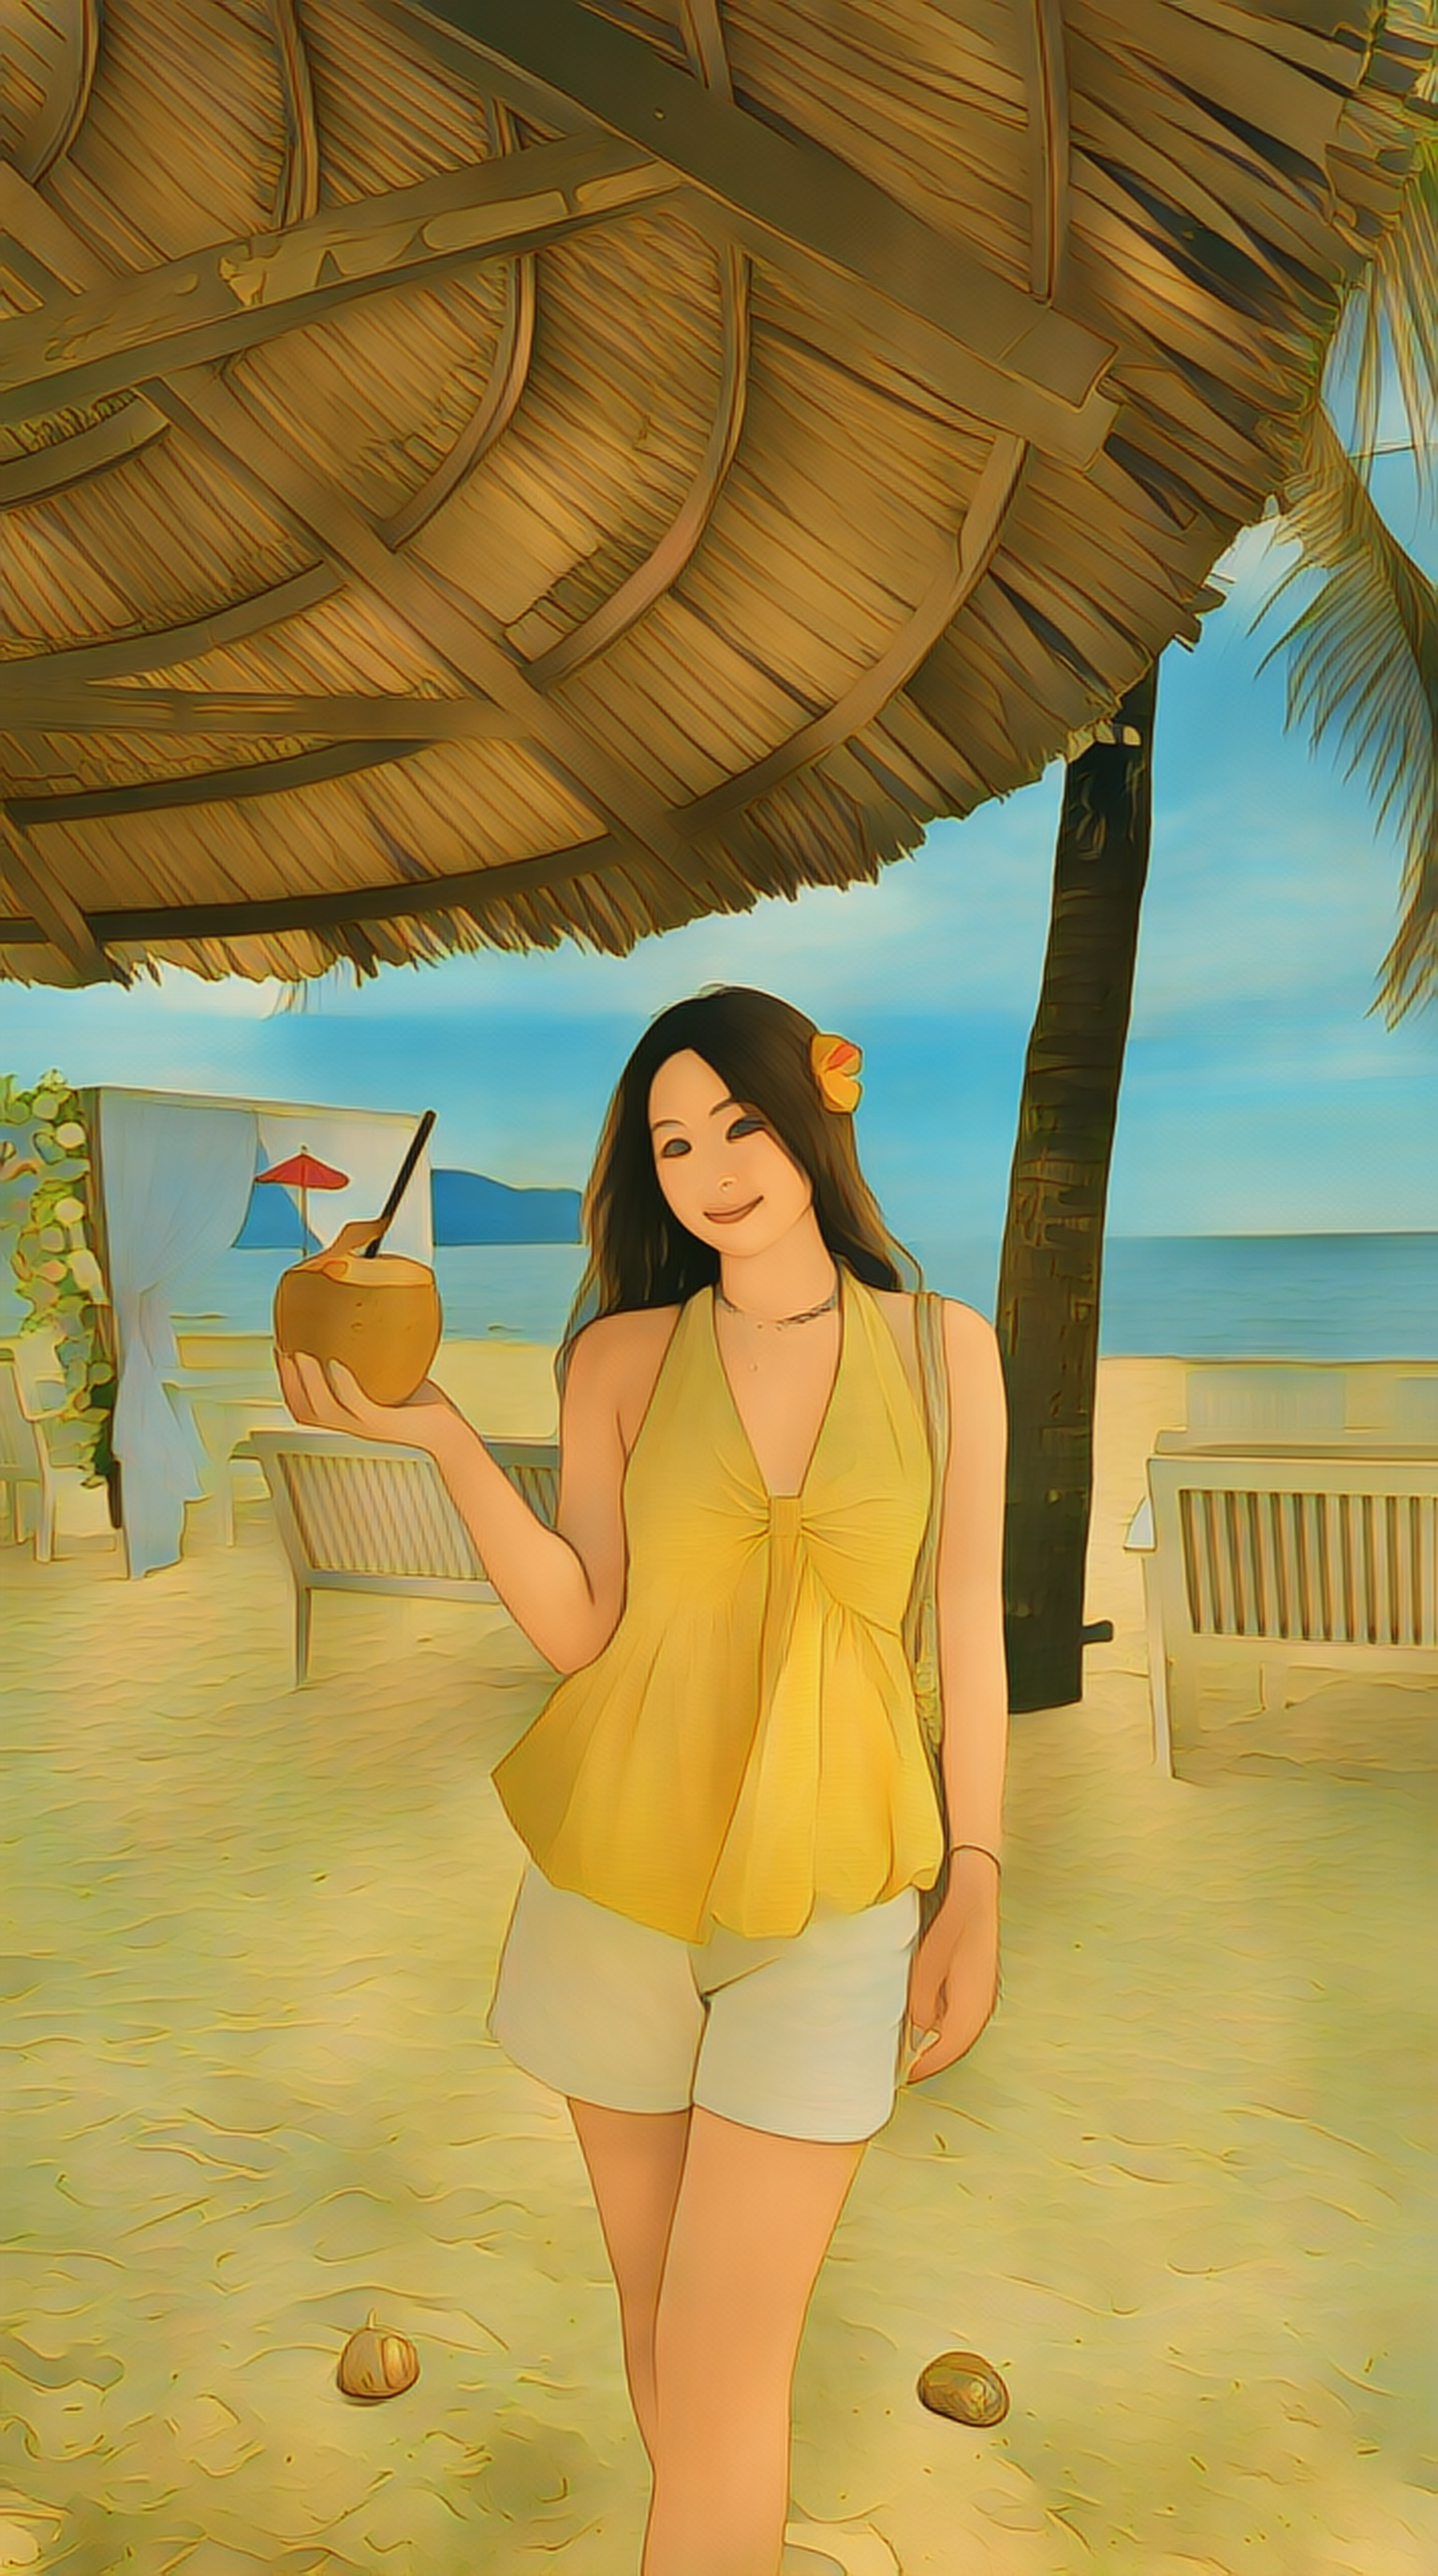
\includegraphics[width=\textwidth]{figChap4/style_results/b1.jpg}
        \caption*{(b) Landscape}
    \end{minipage}
    \hfill
    \begin{minipage}[b]{0.22\textwidth}
        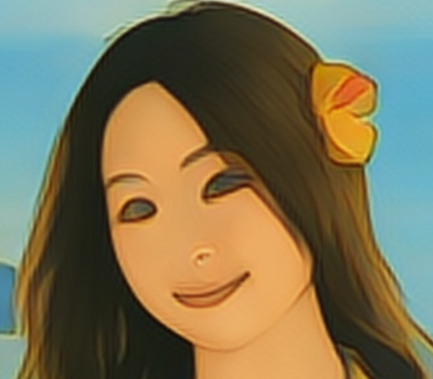
\includegraphics[width=\textwidth]{figChap4/style_results/c1.png}
        \caption*{(c) Cắt mặt từ (b)}
    \end{minipage}
    \hfill
    \begin{minipage}[b]{0.22\textwidth}
        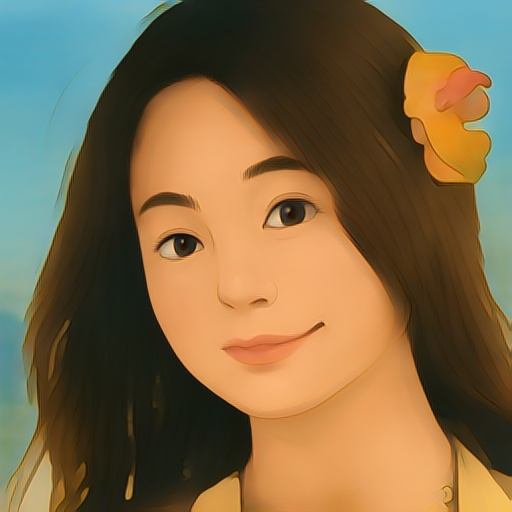
\includegraphics[width=\textwidth]{figChap4/style_results/d1.jpg}
        \caption*{(d) Face Mode}
    \end{minipage}
    \caption{So sánh kết quả chuyển đổi anime giữa Hybrid, Landscape và Face Mode trên ảnh chụp thẳng mặt}
    \label{fig:style_results_1}
\end{figure}
    \noindent\textit{Chú thích:} (a) Hybrid Mode giữ nền anime hóa đồng thời khuôn mặt chất lượng cao nhờ ghép feathered blending. (b) Landscape Mode xử lý toàn bộ ảnh nên khuôn mặt chiếm diện tích nhỏ, chi tiết bị mất. (c) Cắt vùng mặt từ (b) cho thấy đường nét kém sắc. (d) Face Mode tập trung xử lý riêng vùng mặt ($256 \times 256$), cho chi tiết sắc nét nhưng mất nền.

\begin{figure}[H]
    \centering
    \begin{minipage}[b]{0.22\textwidth}
        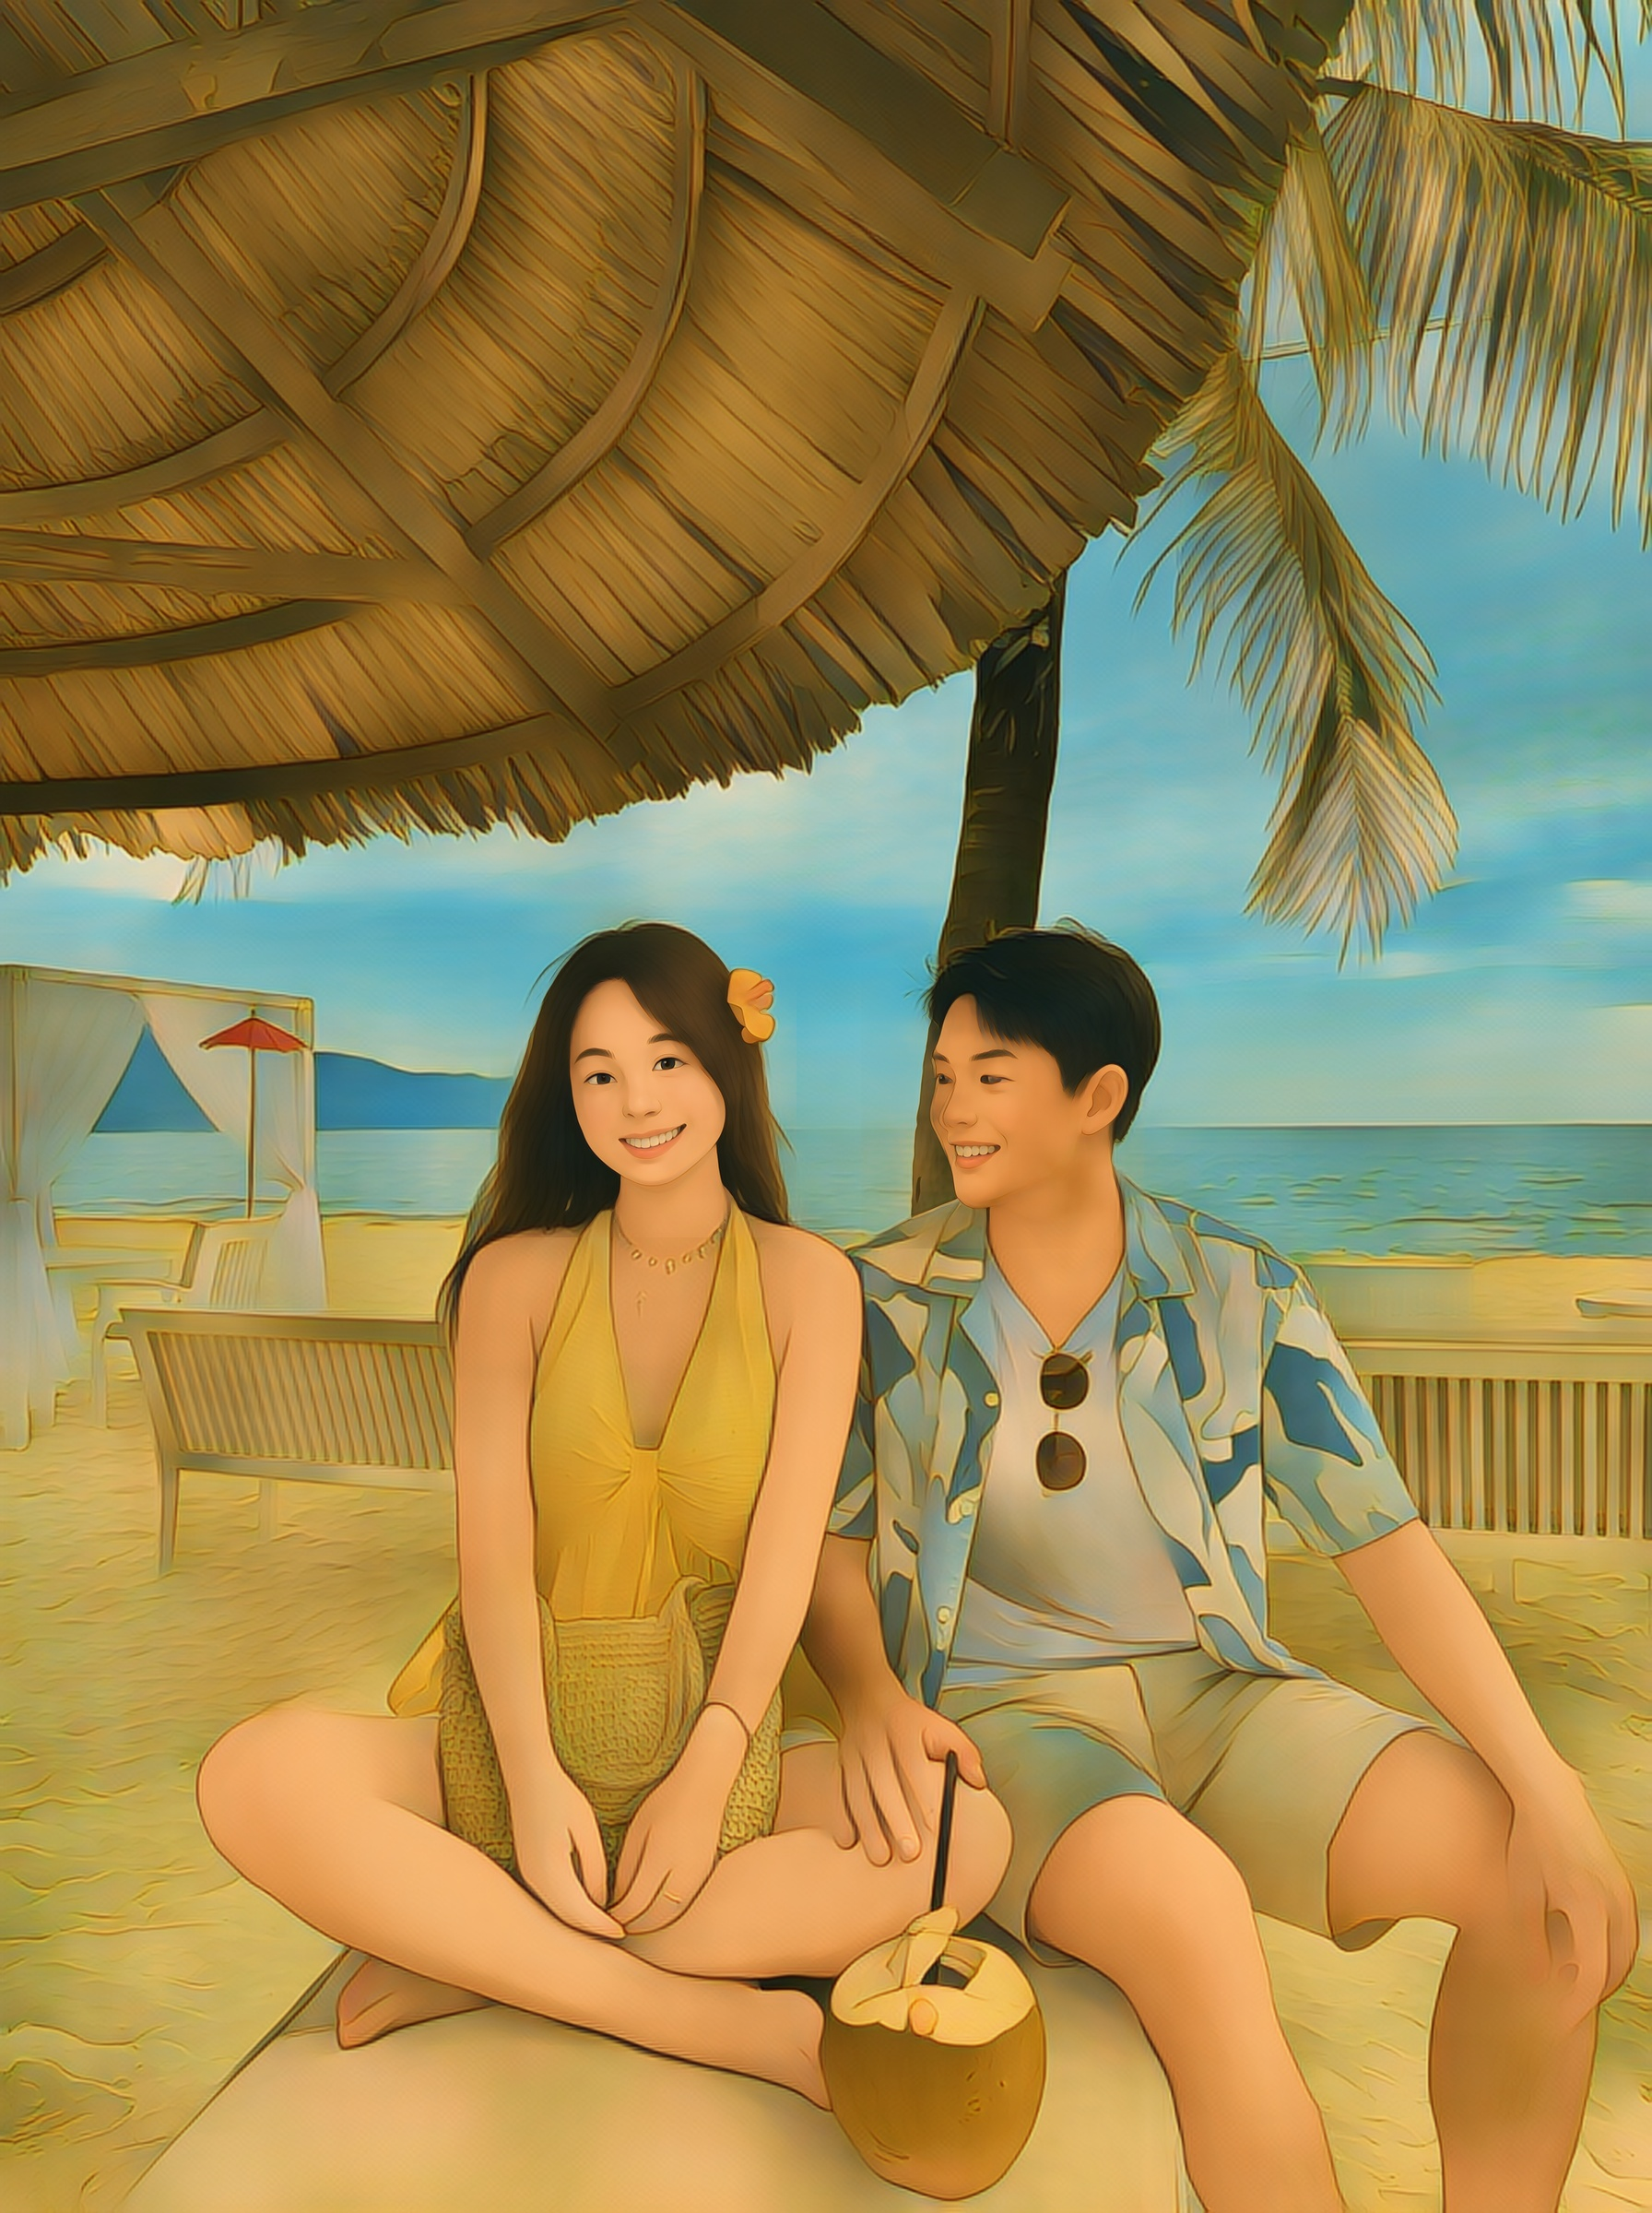
\includegraphics[width=\textwidth]{figChap4/style_results/e2.jpg}
        \caption*{(a) Hybrid}
    \end{minipage}
    \hfill
    \begin{minipage}[b]{0.22\textwidth}
        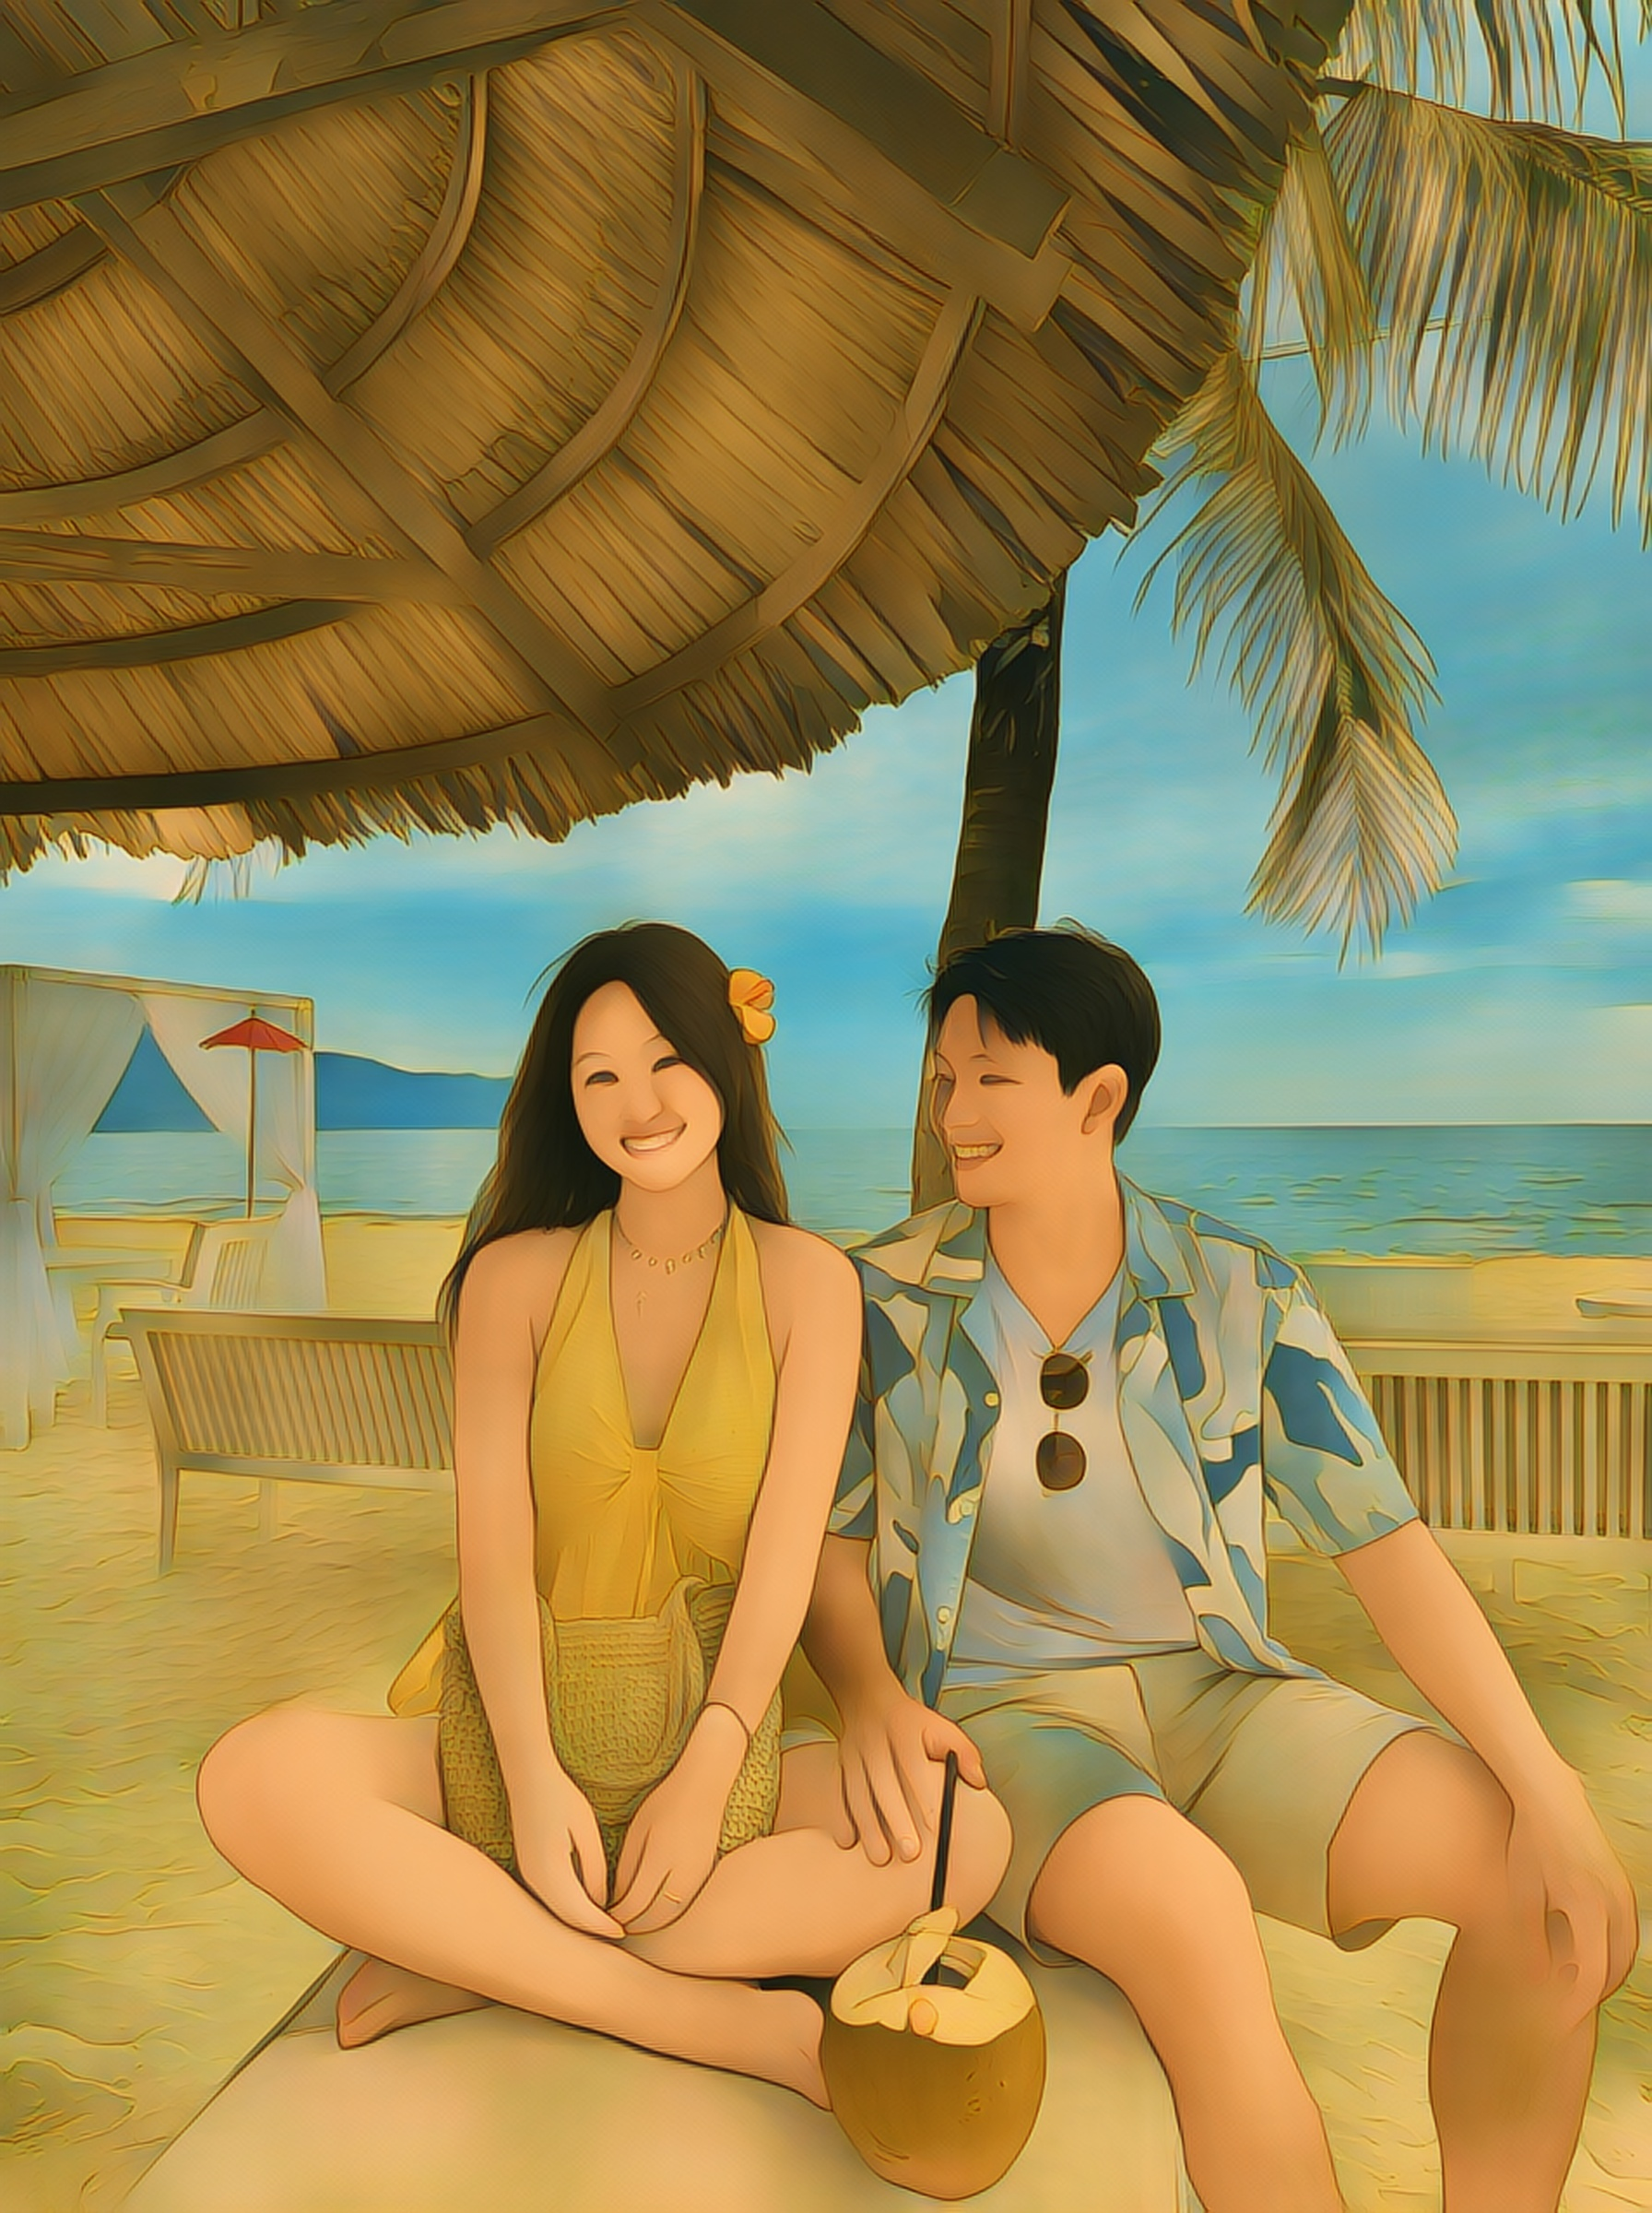
\includegraphics[width=\textwidth]{figChap4/style_results/b2.jpg}
        \caption*{(b) Landscape}
    \end{minipage}
    \hfill
    \begin{minipage}[b]{0.22\textwidth}
        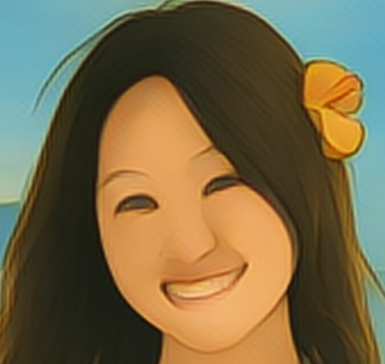
\includegraphics[width=\textwidth]{figChap4/style_results/c2.png}
        \caption*{(c) Cắt mặt từ (b)}
    \end{minipage}
    \hfill
    \begin{minipage}[b]{0.22\textwidth}
        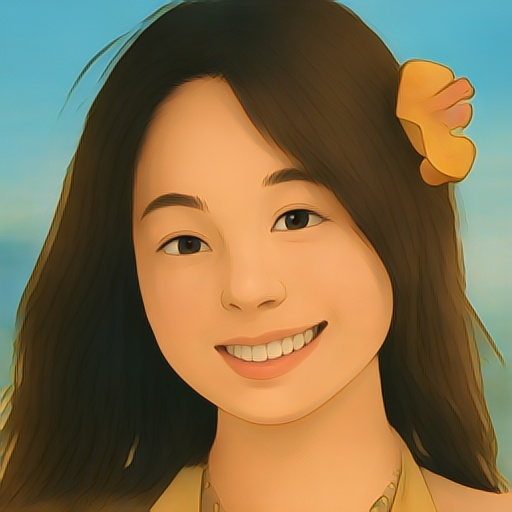
\includegraphics[width=\textwidth]{figChap4/style_results/d2.jpg}
        \caption*{(d) Face Mode}
    \end{minipage}
    \caption{So sánh ba chế độ trên ảnh nhóm người}
    \label{fig:style_results_2}
\end{figure}
    \noindent\textit{Chú thích:} (a) Hybrid Mode xử lý tất cả khuôn mặt phát hiện được ở chất lượng $256 \times 256$ rồi ghép lại nền Landscape --- phù hợp nhất cho ảnh nhóm. (b) Landscape Mode bảo toàn bố cục nhưng chi tiết khuôn mặt bị mất (c). (d) Face Mode chỉ xử lý khuôn mặt lớn nhất, bỏ qua các mặt khác và nền.

\begin{figure}[H]
    \centering
    \begin{minipage}[b]{0.22\textwidth}
        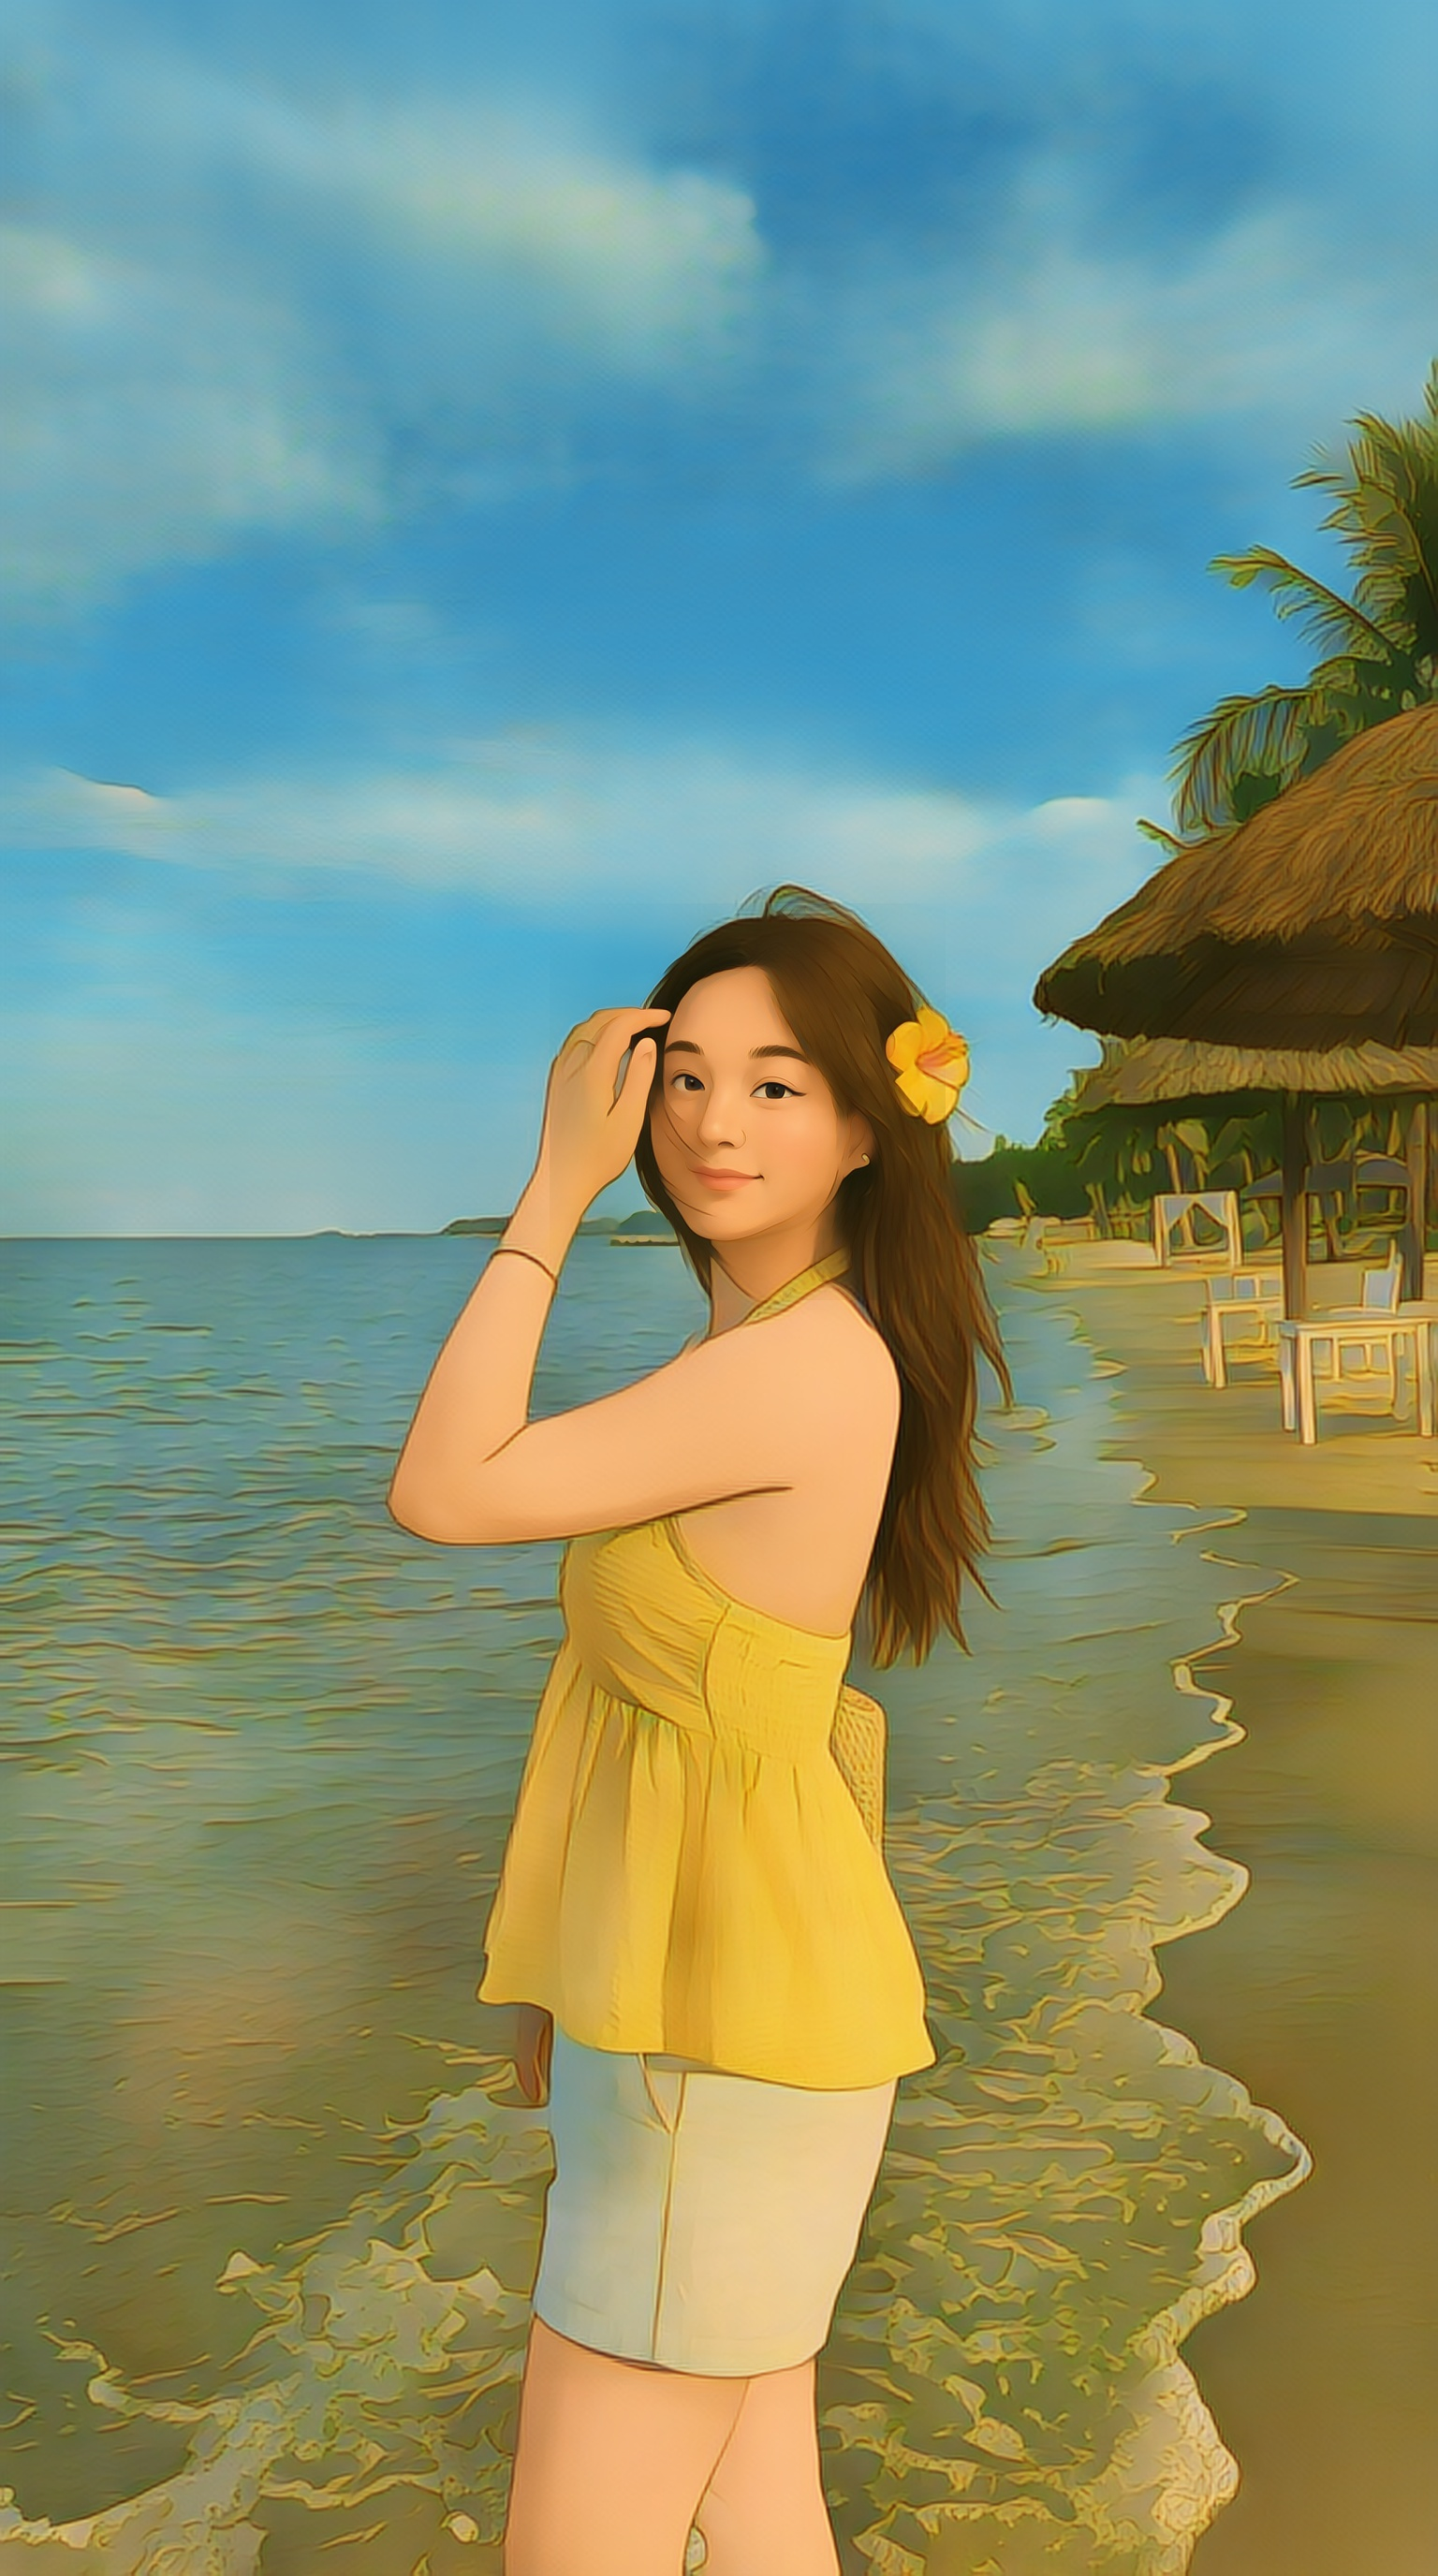
\includegraphics[width=\textwidth]{figChap4/style_results/e3.jpg}
        \caption*{(a) Hybrid}
    \end{minipage}
    \hfill
    \begin{minipage}[b]{0.22\textwidth}
        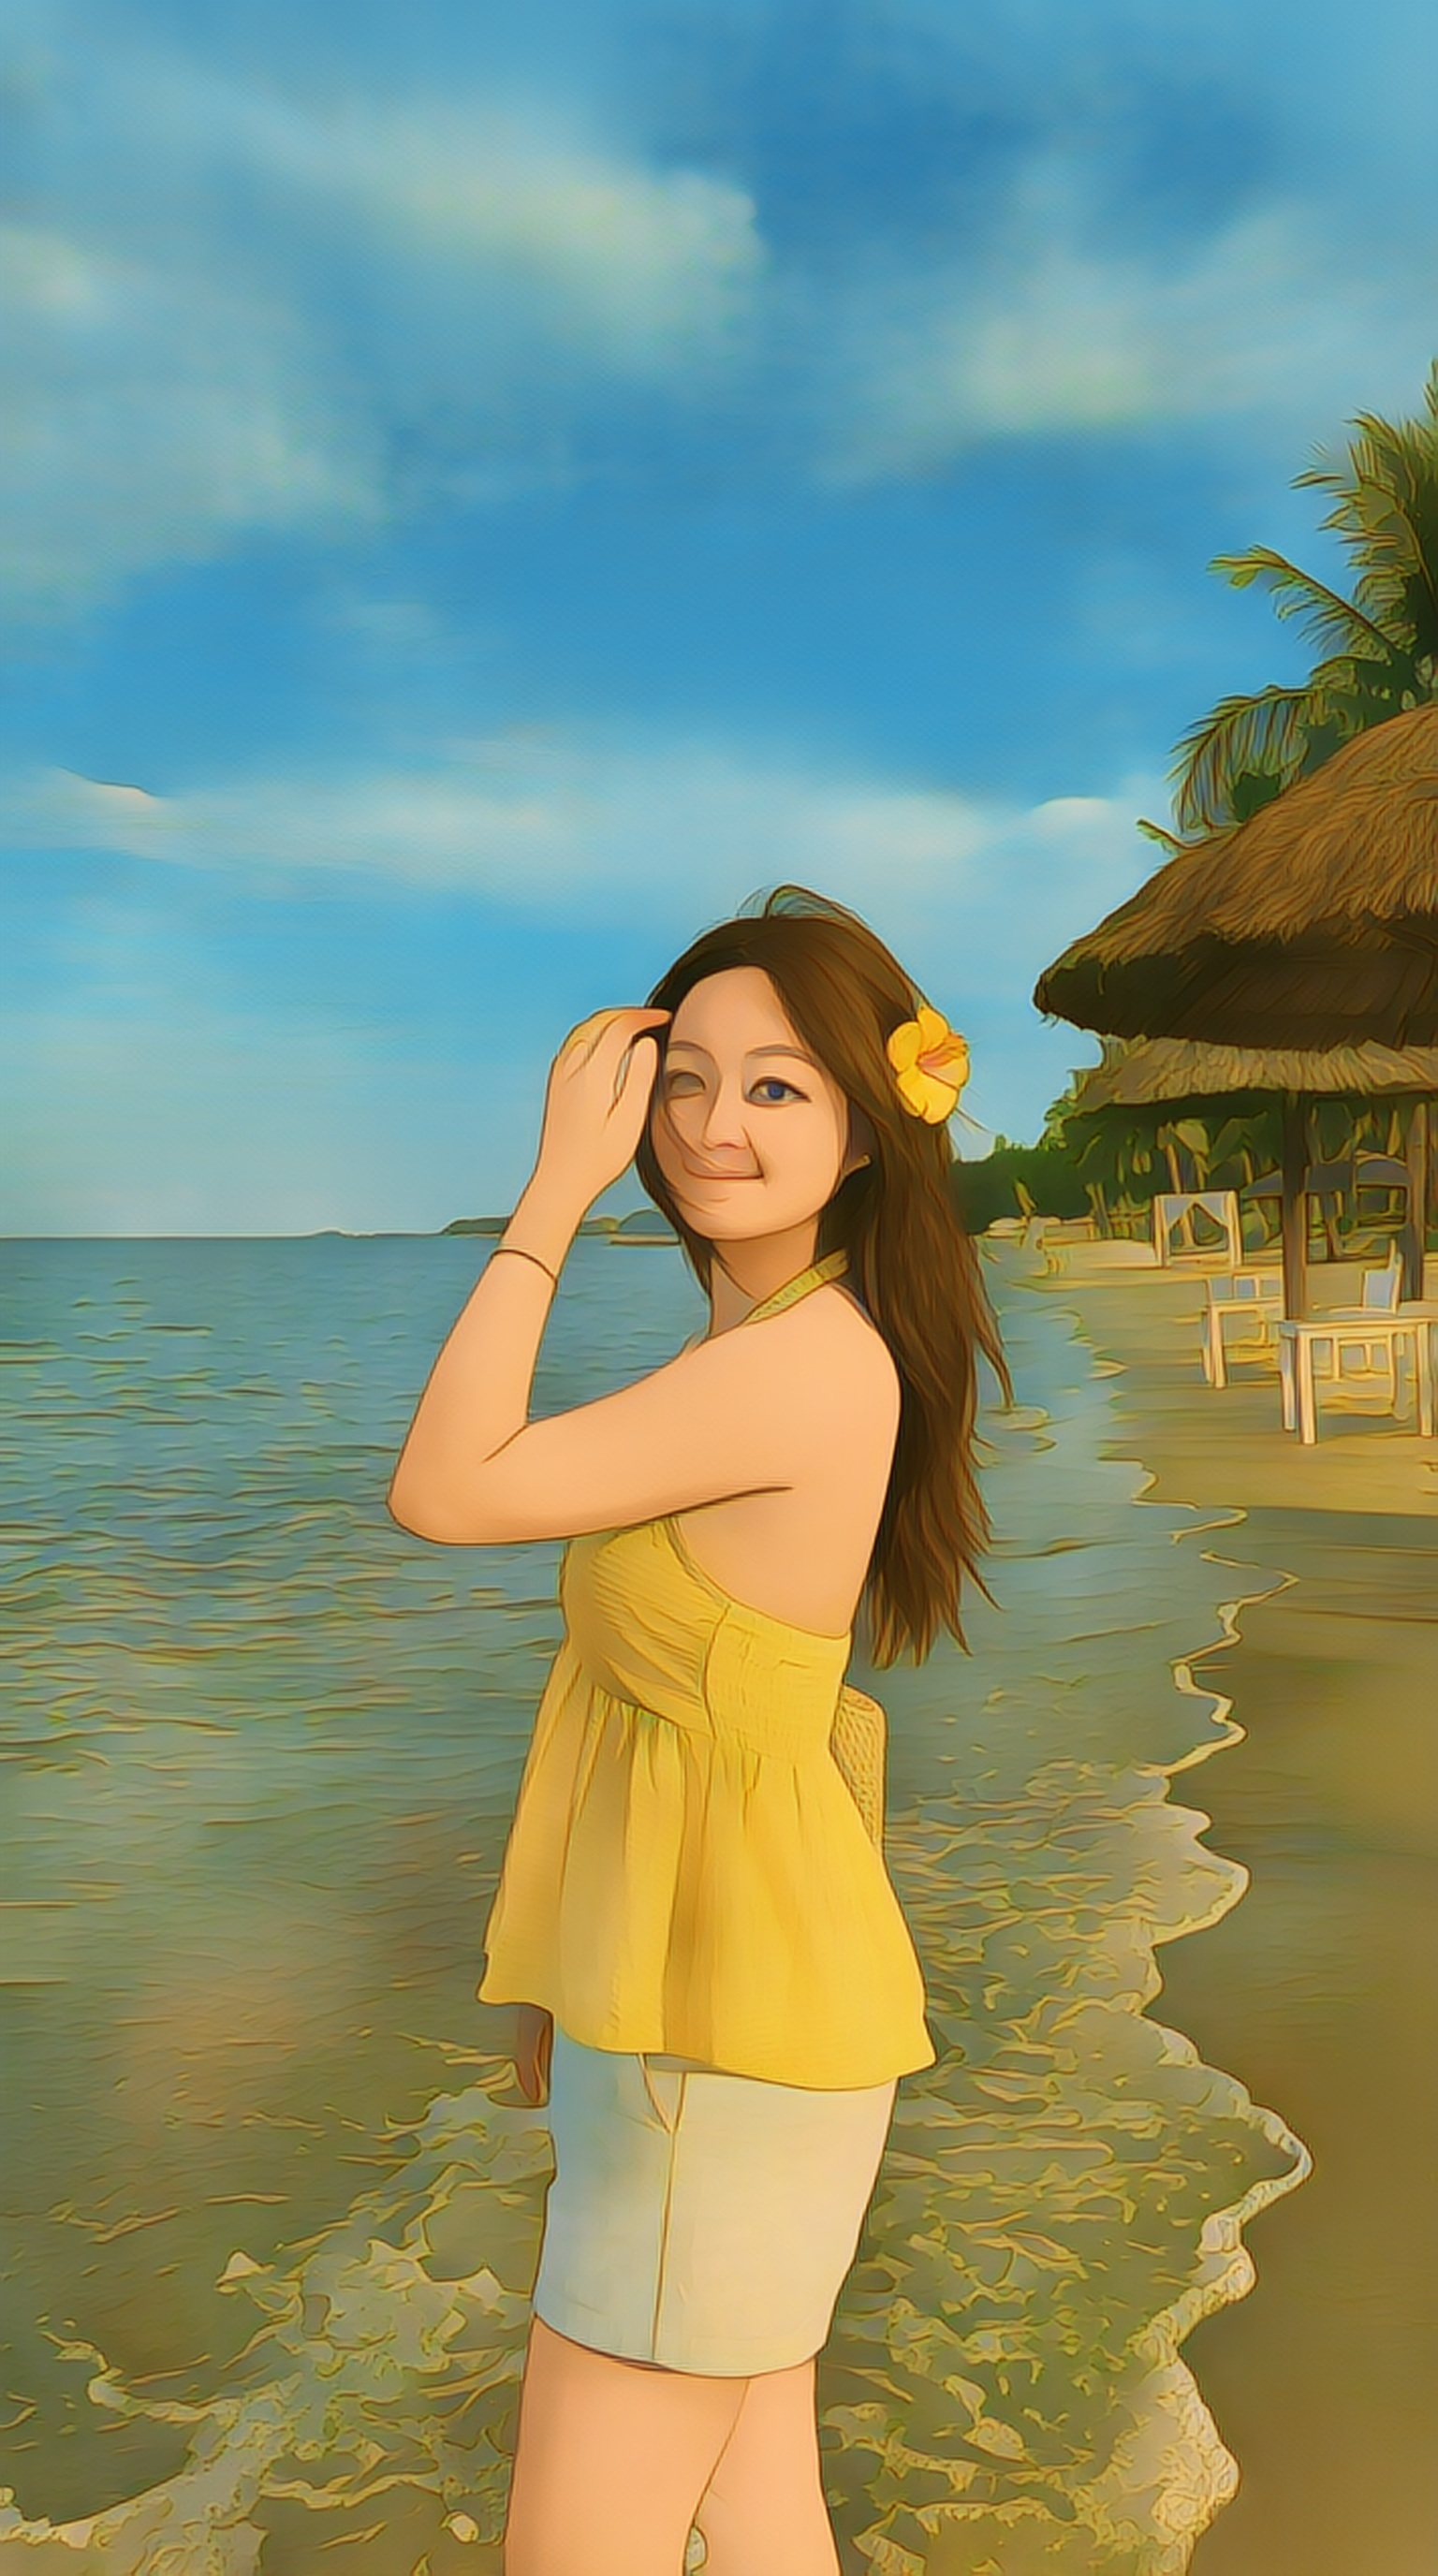
\includegraphics[width=\textwidth]{figChap4/style_results/b3.jpg}
        \caption*{(b) Landscape}
    \end{minipage}
    \hfill
    \begin{minipage}[b]{0.22\textwidth}
        
\includegraphics[width=\textwidth]{figChap4/style_results/c3.png}
        \caption*{(c) Cắt mặt từ (b)}
    \end{minipage}
    \hfill
    \begin{minipage}[b]{0.22\textwidth}
        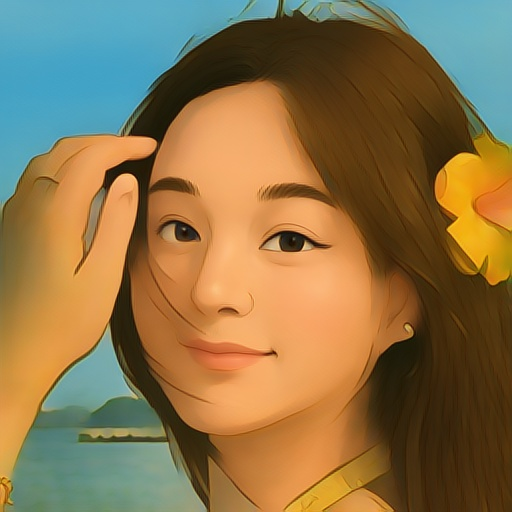
\includegraphics[width=\textwidth]{figChap4/style_results/d3.jpg}
        \caption*{(d) Face Mode}
    \end{minipage}
    \caption{So sánh ba chế độ trên ảnh chân dung góc nghiêng}
    \label{fig:style_results_3}
\end{figure}
    \noindent\textit{Chú thích:} (a) Hybrid Mode giữ nền đồng thời khuôn mặt nghiêng vẫn sắc nét. (d) Face Mode bảo toàn tốt đặc điểm khuôn mặt, làm nhuyễn kết cấu da đặc trưng anime. So với vùng mặt cắt từ Landscape Mode (c), chi tiết ở (a) và (d) sắc nét hơn đáng kể.

\subsection{Phân tích Ảnh hưởng của Module Face Mode}
\label{subsec:face_ext_effect}

\begin{table}[H]
\caption{So sánh chất lượng chuyển đổi giữa ba chế độ xử lý}
\label{tab:face_ext_comparison}
\centering
\begin{tabular}{|p{2.8cm}|p{3.5cm}|p{3.5cm}|p{3.5cm}|}
\hline
\textbf{Tiêu chí} & \textbf{Landscape Mode} & \textbf{Face Mode} & \textbf{Hybrid Mode} \\
\hline
Độ sắc nét mặt & Thấp nếu mặt nhỏ & Cao (mặt chiếm 100\% diện tích) & Cao (từng mặt ở $256^2$) \\
\hline
Bảo toàn chi tiết & Mất chi tiết khi mặt nhỏ & Đầy đủ: mắt, mũi, môi & Đầy đủ cho mọi mặt \\
\hline
Xử lý ảnh nhóm & Tốt (giữ bố cục) & Chỉ mặt lớn nhất & Tất cả khuôn mặt \\
\hline
Background & Giữ nguyên (anime hóa) & Bị cắt bỏ & Giữ (anime hóa) \\
\hline
Số lần suy luận & 1 & 1 & $1 + N$ \\
\hline
FID & 64,2 & \textbf{58,6} & 60,1 \\
\hline
\end{tabular}
\end{table}

Kết quả thực nghiệm khẳng định: Face Mode đạt FID tốt nhất ($58{,}6$, giảm $\approx 8{,}7\%$ so với Landscape Mode) cho ảnh chân dung. Hybrid Mode đạt FID $60{,}1$ --- gần bằng Face Mode nhưng giữ được nền và xử lý tất cả khuôn mặt, phù hợp nhất cho ảnh nhóm người.

\medskip
\noindent\textit{\textbf{Thảo luận --- vì sao Hybrid Mode không bằng Face Mode?} Chênh lệch $1{,}5$ điểm FID giữa Hybrid ($60{,}1$) và Face Mode ($58{,}6$) là một chi tiết đáng phân tích, vì về nguyên tắc vùng khuôn mặt trong hai chế độ được sinh ra bởi \textit{cùng một quy trình}. Có ba nguyên nhân có thể giải thích khoảng cách này, và cả ba đều nằm ở khâu \textbf{ghép ngược}, không phải khâu sinh ảnh. \textbf{Thứ nhất, phép nội suy lại kích thước:} ảnh khuôn mặt được sinh ra ở $256\times256$ rồi resize về kích thước vùng mặt trên ảnh gốc (Chương~3, Mục~\ref{subsec:hybrid_coord_mapping}) --- mọi phép nội suy đều làm suy giảm ít nhiều thành phần tần số cao, tức chính các đường nét sắc mà pipeline đã nỗ lực tạo ra. \textbf{Thứ hai, vùng biên bị pha trộn:} feathered blending làm dải rộng khoảng 8\% mỗi cạnh trở thành trung bình có trọng số giữa đầu ra Face và đầu ra Landscape, nên phần này không đạt chất lượng Face Mode thuần túy. \textbf{Thứ ba, sai số ánh xạ tọa độ} do làm tròn khi quy đổi từ ảnh giới hạn 1280~pixel về ảnh gốc. Nhận định này dẫn tới một hệ quả thực tiễn rõ ràng: muốn thu hẹp khoảng cách $1{,}5$ điểm, cần cải tiến khâu \textbf{ghép} (Poisson blending, mặt nạ bám theo đường viền khuôn mặt) chứ không phải khâu sinh ảnh. Đây là cơ sở cho các đề xuất tại Chương~5.}

% =====================================================
\section{Đánh giá Module Face Mode}
\label{sec:face_extraction_eval}

\subsection{Độ chính xác Phát hiện Khuôn mặt}
\label{subsec:det_accuracy}

Module RetinaFace MobileNet 0.25 được đánh giá độc lập trên tập ảnh kiểm tra gồm các kịch bản khác nhau:

\begin{table}[H]
\caption{Kết quả phát hiện khuôn mặt theo từng kịch bản (ngưỡng confidence = 0,8)}
\label{tab:detection_eval}
\centering
\begin{tabular}{|p{4cm}|c|c|p{4cm}|}
\hline
\textbf{Kịch bản} & \textbf{Precision} & \textbf{Recall} & \textbf{Ghi chú} \\
\hline
Mặt trực diện, ánh sáng tốt & 98,4\% & 97,1\% & Kịch bản lý tưởng \\
\hline
Mặt nghiêng ($<30°$) & 94,2\% & 91,8\% & Hiệu năng giảm nhẹ \\
\hline
Mặt nghiêng ($30°$--$60°$) & 82,7\% & 76,3\% & Giảm đáng kể \\
\hline
Ánh sáng yếu & 88,1\% & 83,5\% & Nhạy cảm với điều kiện chiếu sáng \\
\hline
Mặt nhỏ ($< 32 \times 32$ px) & 71,4\% & 65,9\% & Hạn chế của MobileNet 0.25 \\
\hline
Nhiều khuôn mặt & 95,7\% & -- & Chọn mặt lớn nhất \\
\hline
\end{tabular}
\end{table}

%%% CẦN ĐIỀN: kích thước tập kiểm tra cho từng kịch bản (bao nhiêu ảnh / bao nhiêu khuôn mặt),
%%% nguồn ảnh, và cách gán nhãn ground-truth (tự gán tay hay dùng bộ dữ liệu có sẵn như WIDER FACE?).
%%% Không có thông tin này thì các con số precision/recall không kiểm chứng được.
%%% Ngoài ra, ô Recall của dòng "Nhiều khuôn mặt" đang bỏ trống -- cần điền hoặc giải thích lý do.

Hiệu năng phát hiện cao ở điều kiện thông thường ($>94\%$ precision) và giảm có thể dự đoán ở các điều kiện khó. Đây là hành vi nhất quán với báo cáo trong bài báo gốc RetinaFace \cite{Deng2019RetinaFace}.

Ba xu hướng trong Bảng~\ref{tab:detection_eval} đều có thể lý giải bằng phân tích kiến trúc đã trình bày ở Chương~3:

\begin{itemize}
    \item \textbf{Precision luôn cao hơn Recall} ở mọi kịch bản. Đây là hệ quả trực tiếp của ngưỡng confidence $0{,}8$ --- mức khá cao, được chọn có chủ đích theo nguyên tắc ``bỏ sót còn hơn nhầm lẫn'' đã phân tích tại Chương~3 (Mục~\ref{subsec:retinaface_postprocess}). Kết quả thực nghiệm xác nhận rằng lựa chọn này hoạt động đúng như thiết kế.
    \item \textbf{Suy giảm mạnh với mặt nhỏ hơn $32\times32$~px} (precision $71{,}4\%$). Nguyên nhân đã được nêu tại Chương~3: dù các anchor tầng $P_3$ phủ tới kích thước 16~px, backbone MobileNet~0.25 với chỉ 25\% số kênh không đủ dung lượng biểu diễn để phân biệt khuôn mặt rất nhỏ với nhiễu có cấu trúc.
    \item \textbf{Suy giảm theo góc nghiêng} có tính hai bậc: dưới $30°$ gần như không ảnh hưởng ($94{,}2\%$), nhưng từ $30°$ đến $60°$ giảm mạnh xuống $82{,}7\%$. Đây chính là nhóm ảnh mà kỹ thuật face alignment dựa trên 5 landmark --- hiện chưa được khai thác (Chương~3, Mục~\ref{subsec:margin_value}) --- có tiềm năng cải thiện lớn nhất.
\end{itemize}

\medskip
\noindent\textit{\textbf{Nhận xét về tác động thực tế của lỗi phát hiện:} Điều quan trọng cần đặt các con số trên vào đúng bối cảnh là \textbf{hậu quả của hai loại lỗi rất khác nhau} trong hệ thống này. Một lần bỏ sót (recall giảm) chỉ khiến hệ thống hạ cấp mềm về Landscape Mode --- người dùng vẫn nhận được kết quả hợp lệ, chỉ là khuôn mặt kém sắc nét hơn. Ngược lại, một lần phát hiện nhầm (precision giảm) sẽ khiến một vùng nền ngẫu nhiên bị anime hóa như khuôn mặt rồi dán đè lên ảnh --- lỗi thị giác rõ rệt và gây khó chịu. Với cấu hình hiện tại, precision được giữ ở mức cao ($\geq 88\%$ ở mọi kịch bản trừ mặt rất nhỏ), tức hệ thống đang ưu tiên đúng loại lỗi ít gây hại hơn. Đây là một ví dụ cho thấy việc chọn ngưỡng trong hệ thống thực tế cần dựa trên \textbf{chi phí của từng loại lỗi} chứ không phải trên việc tối đa hóa một chỉ số tổng hợp như F1-score.}

\subsection{Phân tích Tham số margin}
\label{subsec:margin_analysis}

Thực nghiệm so sánh 3 giá trị tham số margin khác nhau trên tập 50 ảnh chân dung:

\begin{table}[H]
\caption{Ảnh hưởng của tham số margin đến chất lượng ảnh đầu ra và mức độ bao phủ ngữ cảnh}
\label{tab:margin_eval}
\centering
\begin{tabular}{|c|c|c|c|p{5.5cm}|}
\hline
\textbf{margin $m$} & \textbf{$w_{\text{model}}$} & \textbf{FID $\downarrow$} & \textbf{LPIPS} & \textbf{Nhận định định tính} \\
\hline
0,3 & 160 px & 63,1 & 0,401 & Thường cắt mất tóc và tai; khuôn mặt cứng, thiếu ngữ cảnh \\
\hline
\textbf{0,5} & \textbf{128 px} & \textbf{58,6} & \textbf{0,384} & Cân bằng tốt; bao gồm tóc, tai, cổ; ảnh anime tự nhiên nhất \\
\hline
0,7 & 107 px & 61,3 & 0,396 & Bao quá nhiều nền; phong cách bị nhiễu bởi background \\
\hline
\end{tabular}
\end{table}

Cột $w_{\text{model}}$ được bổ sung để làm rõ cơ chế đằng sau kết quả: theo Tính chất 3 đã chứng minh ở Chương~3 (Phương trình~\ref{eq:face_width_after}), bề rộng khuôn mặt trong ảnh đưa vào Generator là $w_{\text{model}} = 256/(1+2m)$, tức giảm đơn điệu khi $m$ tăng.

Kết quả cho thấy quan hệ giữa $m$ và FID có dạng \textbf{hình chữ U}, với cực tiểu tại $m = 0{,}5$. Điều này xác nhận đúng cơ chế đánh đổi hai chiều đã dự đoán ở Chương~3 (Mục~\ref{subsec:margin_value}):

\begin{itemize}
    \item \textbf{Nhánh trái ($m = 0{,}3$, FID $63{,}1$):} khuôn mặt được xử lý ở độ phân giải cao nhất (160~px) nhưng vùng cắt thiếu tóc và tai --- một dạng đầu vào \textit{ngoài phân phối huấn luyện}. Độ phân giải cao không bù đắp được cho việc mô hình gặp loại dữ liệu chưa từng thấy.
    \item \textbf{Nhánh phải ($m = 0{,}7$, FID $61{,}3$):} vùng cắt có đủ ngữ cảnh nhưng khuôn mặt chỉ còn 107~px, đồng thời nền chiếm tỉ lệ lớn và chi phối các thống kê toàn cục mà LADE cùng External Attention sử dụng.
\end{itemize}

Điểm cân bằng $m = 0{,}5$ được giữ cố định làm tham số mặc định trong ứng dụng. LPIPS biến thiên cùng chiều với FID trên cả ba cấu hình, cho thấy hai chỉ số nhất quán với nhau ở thí nghiệm này.

\medskip
\noindent\textit{\textbf{Nhận xét về độ tin cậy:} Cần ghi nhận rằng thí nghiệm này được thực hiện trên tập chỉ \textbf{50 ảnh} --- nhỏ hơn nhiều so với tập 1.000 ảnh dùng cho các chỉ số chính. Với cỡ mẫu này, chỉ số FID có phương sai ước lượng đáng kể, và chênh lệch $4{,}5$ điểm giữa $m = 0{,}3$ và $m = 0{,}5$ tuy rõ ràng nhưng chênh lệch $2{,}7$ điểm giữa $m = 0{,}5$ và $m = 0{,}7$ thì kém chắc chắn hơn. Kết luận an toàn có thể rút ra là: \textbf{$m$ nằm trong khoảng $0{,}5$--$0{,}7$ đều cho kết quả chấp nhận được, còn $m = 0{,}3$ rõ ràng là quá nhỏ}. Để khẳng định $m = 0{,}5$ là tối ưu, cần lặp lại thí nghiệm trên tập lớn hơn và khảo sát lưới giá trị mịn hơn (chẳng hạn $m \in \{0{,}4;\ 0{,}5;\ 0{,}6\}$).}

\subsection{Xử lý Trường hợp Đặc biệt}
\label{subsec:edge_cases_eval}

\begin{table}[H]
\caption{Kết quả xử lý các trường hợp đặc biệt trong module Face Mode}
\label{tab:edge_cases}
\centering
\begin{tabular}{|p{3.5cm}|p{4.5cm}|p{5cm}|}
\hline
\textbf{Trường hợp} & \textbf{Hành vi hệ thống} & \textbf{Kết quả} \\
\hline
Không phát hiện mặt & Tự động chuyển Landscape Mode & Toàn bộ ảnh được xử lý \\
\hline
Nhiều khuôn mặt (Face Mode) & Chọn khuôn mặt lớn nhất & Mặt chủ thể được ưu tiên \\
\hline
Nhiều khuôn mặt (Hybrid Mode) & Xử lý tất cả khuôn mặt & Mọi mặt đều chất lượng cao \\
\hline
Khuôn mặt gần biên & Margin Expansion đối xứng với lề thu hẹp & Vùng cắt hợp lệ trong biên ảnh \\
\hline
Ảnh chụp xa (long shot) & Mặt nhỏ, confidence $<$ 0,8 & Hạ cấp mềm sang Landscape Mode \\
\hline
Góc nghiêng $>60°$ & Bounding box không chính xác & Kết quả kém; cần face alignment \\
\hline
\end{tabular}
\end{table}

Bảng trên xác nhận rằng cơ chế hạ cấp mềm hoạt động đúng thiết kế trong mọi tình huống được kiểm tra: hệ thống không trả về lỗi trong bất kỳ trường hợp nào, mà luôn cho ra một kết quả hợp lệ dù có thể không tối ưu. Trường hợp duy nhất cho kết quả thực sự kém là góc nghiêng lớn hơn $60°$ --- đúng nhóm mà cả Bảng~\ref{tab:detection_eval} lẫn phân tích ở Chương~3 đều đã dự báo.

% =====================================================
\section{Đánh giá Người dùng (User Study)}
\label{sec:user_study}

\subsection{Thiết kế Khảo sát}
\label{subsec:user_study_design}

Để đánh giá chất lượng cảm nhận của hệ thống từ góc độ người dùng thực tế, một nghiên cứu khảo sát có cấu trúc đã được tiến hành với \textbf{42 người tham gia}, chia thành hai nhóm:
\begin{itemize}
    \item \textbf{Chuyên gia} ($n = 12$): Nhà thiết kế đồ họa, họa sĩ kỹ thuật số, giảng viên nghệ thuật.
    \item \textbf{Người dùng phổ thông} ($n = 30$): Người dùng không có nền tảng chuyên môn về đồ họa.
\end{itemize}

Mỗi người tham gia được yêu cầu đánh giá các cặp ảnh (đầu ra Hybrid Mode so với Landscape Mode) theo thang Likert 5 điểm trên ba tiêu chí:
\begin{enumerate}
    \item Mức độ bảo toàn danh tính khuôn mặt (facial identity preservation).
    \item Độ sắc nét của các chi tiết khuôn mặt (visual sharpness).
    \item Độ tự nhiên tổng thể của kết quả anime (overall naturalness).
\end{enumerate}

%%% CẦN BỔ SUNG (hội đồng thường hỏi các mục này):
%%%  - Mỗi người đánh giá BAO NHIÊU cặp ảnh?
%%%  - Các cặp ảnh được chọn thế nào (ngẫu nhiên / có chủ đích)?
%%%  - Thứ tự trái/phải của hai ảnh trong mỗi cặp có được xáo trộn ngẫu nhiên không?
%%%    (nếu không, kết quả có thể bị thiên lệch vị trí)
%%%  - Người tham gia có biết ảnh nào thuộc phương pháp nào không (khảo sát mù?)
%%%  - Hình thức khảo sát (trực tuyến / trực tiếp), thời gian thực hiện
%%%  - Người tham gia có được thông báo và đồng ý tham gia không

\subsection{Kết quả}
\label{subsec:user_study_results}

\begin{table}[H]
\caption{Kết quả đánh giá cảm nhận người dùng: Hybrid Mode so với Landscape Mode (thang Likert 5 điểm, $n = 42$)}
\label{tab:user_study}
\centering
\begin{tabular}{|p{5cm}|c|c|}
\hline
\textbf{Tiêu chí} & \textbf{Điểm TB $\pm$ SD} & \textbf{Tỉ lệ ưu tiên Hybrid} \\
\hline
Bảo toàn danh tính khuôn mặt & $3{,}7 \pm 1{,}1$ & -- \\
\hline
Độ sắc nét chi tiết khuôn mặt & $3{,}4 \pm 1{,}1$ & 88,8\% \\
\hline
Độ tự nhiên tổng thể & $3{,}7 \pm 1{,}1$ & 88,8\% \\
\hline
\end{tabular}
\end{table}

%%% CẦN KIỂM TRA LẠI SỐ LIỆU: ba giá trị SD đều bằng 1,1 và hai tỉ lệ ưu tiên đều bằng 88,8%.
%%% Sự trùng lặp này có thể là ngẫu nhiên, nhưng cũng có thể là lỗi sao chép khi lập bảng.
%%% Hãy đối chiếu lại với dữ liệu khảo sát thô.
%%% Ngoài ra, ô "Tỉ lệ ưu tiên" của tiêu chí đầu tiên đang bỏ trống -- cần điền hoặc
%%% giải thích vì sao tiêu chí này không có so sánh ưu tiên.

Kết quả cho thấy Hybrid Mode nhận được đánh giá tích cực ở cả ba tiêu chí, với điểm trung bình từ $3{,}4$ đến $3{,}7$ trên thang 5 --- đều cao hơn mức trung tính $3{,}0$. Trong các so sánh trực tiếp về độ sắc nét và tính tự nhiên của khuôn mặt, người tham gia \textbf{ưu tiên Hybrid Mode hơn Landscape Mode trong 88,8\% trường hợp}.

\textbf{Kiểm định thống kê:} Bài kiểm định Wilcoxon signed-rank test trên các đánh giá ghép cặp theo ảnh xác nhận Hybrid Mode được ưu tiên hơn Landscape Mode có ý nghĩa thống kê trên cả ba tiêu chí ($p < 0{,}001$, $n = 42$). Bài kiểm định Mann-Whitney U giữa nhóm Chuyên gia và Người dùng phổ thông không cho thấy sự khác biệt đáng kể ($p > 0{,}75$).

\textbf{Lý do chọn kiểm định phi tham số.} Dữ liệu thang Likert là dữ liệu \textit{thứ bậc} (ordinal): khoảng cách giữa mức 1 và mức 2 không nhất thiết bằng khoảng cách giữa mức 4 và mức 5. Các kiểm định tham số như $t$-test giả định dữ liệu ở thang khoảng (interval) và phân phối chuẩn --- những giả định không thỏa mãn ở đây. Wilcoxon signed-rank test (cho dữ liệu ghép cặp) và Mann-Whitney U test (cho hai nhóm độc lập) chỉ dựa trên thứ hạng, nên phù hợp hơn với loại dữ liệu này.

\medskip
\noindent\textit{\textbf{Thảo luận:} Kết quả kiểm định Mann-Whitney U giữa hai nhóm ($p > 0{,}75$) là phát hiện đáng chú ý nhất của khảo sát, và cần được diễn giải cẩn thận. Việc \textbf{không bác bỏ} giả thuyết không đồng nghĩa với việc \textbf{chứng minh} hai nhóm giống nhau --- với cỡ mẫu 12 chuyên gia, năng lực thống kê (statistical power) để phát hiện khác biệt nhỏ là khá thấp. Cách phát biểu chặt chẽ là: \textit{dữ liệu hiện có không đủ bằng chứng để kết luận chuyên gia đánh giá khác người dùng phổ thông}. Dù vậy, kết quả này vẫn có giá trị thực tiễn: nếu cải thiện chất lượng do Hybrid Mode mang lại chỉ có chuyên gia mới nhận ra, giá trị ứng dụng của hệ thống sẽ hạn chế; việc cả hai nhóm phản ứng tương tự nhau gợi ý rằng cải thiện đủ rõ để người dùng thông thường cảm nhận được. Một điểm khác đáng lưu ý là tiêu chí ``độ sắc nét'' có điểm trung bình thấp nhất ($3{,}4$) trong ba tiêu chí, dù đây chính là khía cạnh mà Face Mode được thiết kế để cải thiện. Điều này nhất quán với phân tích tại Mục~\ref{subsec:face_ext_effect}: trong Hybrid Mode, khuôn mặt phải trải qua thêm một lần nội suy lại kích thước và một vùng biên bị pha trộn, làm suy giảm chính độ sắc nét mà nó tạo ra. Đây là bằng chứng độc lập --- từ cảm nhận người dùng thay vì từ chỉ số tự động --- củng cố cho kết luận rằng khâu \textbf{ghép} là nút thắt cần cải tiến tiếp theo.}

% =====================================================
\iffalse % Tạm thời comment phần 4.9 theo yêu cầu
\section{Triển khai Ứng dụng Web}
\label{sec:web_app}

Để minh chứng khả năng ứng dụng thực tiễn của hệ thống, luận văn đã xây dựng một ứng dụng web hoàn chỉnh cho phép người dùng tải ảnh lên và nhận kết quả anime hóa theo cả ba chế độ.

\subsection{Kiến trúc Hệ thống}
\label{subsec:webapp_arch}

Ứng dụng được tổ chức theo kiến trúc client--server tách biệt:

\begin{itemize}
    \item \textbf{Frontend (React 19):} Giao diện người dùng cho phép tải ảnh, chọn phong cách và chế độ xử lý, xem trước kết quả và tải về. Toàn bộ xử lý ảnh được thực hiện ở phía máy chủ; frontend chỉ đảm nhiệm việc hiển thị và tương tác.
    \item \textbf{Backend (FastAPI):} Cung cấp các điểm cuối (endpoint) REST nhận ảnh, điều phối pipeline đã trình bày ở Chương~3, và trả về kết quả. FastAPI được chọn nhờ hỗ trợ xử lý bất đồng bộ (async) --- phù hợp với tác vụ suy luận có độ trễ đáng kể --- và khả năng tự sinh tài liệu API.
    \item \textbf{Lớp suy luận (ONNX Runtime):} Nạp sẵn các phiên suy luận (session) của RetinaFace và AnimeGANv3 khi khởi động máy chủ, tránh chi phí nạp lại mô hình cho mỗi yêu cầu.
\end{itemize}

\begin{figure}[H]
    \centering
    \includegraphics[width=0.9\textwidth]{figChap4/webapp_architecture.png}
    \caption{Kiến trúc ứng dụng web: React frontend, FastAPI backend và lớp suy luận ONNX Runtime}
    \label{fig:webapp_arch}
\end{figure}

%%% CẦN BỔ SUNG HÌNH: figChap4/webapp_architecture.png -- sơ đồ khối kiến trúc ứng dụng.

\subsection{Giao diện và Luồng Sử dụng}
\label{subsec:webapp_ui}

\begin{figure}[H]
    \centering
    \includegraphics[width=0.9\textwidth]{figChap4/webapp_ui.png}
    \caption{Giao diện ứng dụng web: khu vực tải ảnh, bảng chọn phong cách và chế độ, khung xem kết quả}
    \label{fig:webapp_ui}
\end{figure}

%%% CẦN BỔ SUNG HÌNH: figChap4/webapp_ui.png -- ảnh chụp màn hình giao diện.
%%% Nên có 2-3 ảnh: màn hình chính, màn hình đang xử lý, màn hình kết quả.

Luồng sử dụng gồm bốn bước: (1) người dùng tải ảnh lên; (2) chọn phong cách anime và chế độ xử lý; (3) hệ thống thực hiện pipeline và hiển thị tiến trình; (4) hiển thị kết quả kèm nút tải về. Hệ thống hỗ trợ cả ảnh đơn và xử lý theo lô, cũng như chuyển đổi video theo từng khung hình.

\subsection{Hiệu năng Đầu-cuối}
\label{subsec:webapp_perf}

\begin{table}[H]
\caption{Thời gian phản hồi đầu-cuối của ứng dụng web (ảnh $1280 \times 960$, GPU RTX A5000)}
\label{tab:webapp_perf}
\centering
\begin{tabular}{|l|c|c|c|}
\hline
\textbf{Chế độ} & \textbf{Phát hiện mặt} & \textbf{Suy luận} & \textbf{Tổng thời gian} \\
\hline
Landscape Mode & -- & \textbf{[cần đo]} & \textbf{[cần đo]} \\
\hline
Face Mode & \textbf{[cần đo]} & \textbf{[cần đo]} & \textbf{[cần đo]} \\
\hline
Hybrid Mode ($N=1$) & \textbf{[cần đo]} & \textbf{[cần đo]} & \textbf{[cần đo]} \\
\hline
Hybrid Mode ($N=3$) & \textbf{[cần đo]} & \textbf{[cần đo]} & \textbf{[cần đo]} \\
\hline
\end{tabular}
\end{table}

%%% CẦN ĐO VÀ ĐIỀN BẢNG TRÊN. Cách đo đơn giản: thêm log thời gian ở backend cho từng
%%% giai đoạn (đọc ảnh, phát hiện, suy luận, ghép, mã hóa trả về), chạy 20 lần rồi lấy trung bình.
%%% Bảng này rất có giá trị vì nó kiểm chứng trực tiếp công thức độ phức tạp
%%% T_hybrid = T_D + T_L + N*T_F ở Chương 3 (Phương trình eq:hybrid_time).
%%% Nếu số liệu khớp với công thức, đó là một minh chứng thực nghiệm mạnh.

Cần lưu ý rằng thời gian phản hồi đầu-cuối lớn hơn thời gian suy luận thuần túy báo cáo ở Mục~\ref{subsec:inference_speed}, do bao gồm thêm các chi phí truyền tải mạng, giải mã và mã hóa ảnh, cùng các thao tác tiền/hậu xử lý trên CPU.
\fi

% =====================================================
\section{Thảo luận và Phân tích}
\label{sec:discussion}

\subsection{Điểm mạnh của Hệ thống}
\label{subsec:strengths}

Hệ thống đạt được nhiều điểm mạnh đáng chú ý. Về chất lượng ảnh đầu ra, chỉ số FID $58{,}6$ ở chế độ Face Mode cho thấy phân phối ảnh sinh ra gần với ảnh anime thật hơn đáng kể so với các phương pháp đối chứng như CycleGAN (FID $98{,}4$) và CartoonGAN (FID $84{,}7$). Đồng thời, hệ thống đạt hiệu năng cao với 42~FPS ở độ phân giải $256\times256$ trên GPU và model size chỉ $9{,}1$~MB ONNX, phù hợp cho triển khai thực tế.

Về mặt kiến trúc, các phân tích thực nghiệm trong chương này cung cấp bằng chứng ủng hộ cho một số lập luận thiết kế đã nêu ở các chương trước:

\begin{itemize}
    \item Việc lựa chọn LSGAN thay vì entropy chéo được xác nhận qua việc Generator tiếp tục học ổn định dù D\_loss ở mức thấp (Mục~\ref{subsec:full_training_results}).
    \item Sự đánh đổi giữa mục tiêu phong cách và mục tiêu nội dung --- được mô hình hóa bằng Phương trình~(\ref{eq:conflict_objective}) ở Chương~2 --- được quan sát trực tiếp qua xu hướng ngược chiều của sty\_loss và con\_loss theo epoch.
    \item Quan hệ hình chữ U giữa tham số $m$ và FID (Mục~\ref{subsec:margin_analysis}) khớp với cơ chế đánh đổi hai chiều đã dự đoán ở Chương~3.
\end{itemize}

\subsection{Hạn chế và Định hướng Cải thiện}
\label{subsec:limitations}

Bên cạnh những điểm mạnh, hệ thống vẫn còn một số hạn chế cần lưu ý:

\begin{enumerate}
    \item \textbf{Phụ thuộc vào tập dữ liệu phong cách.} Chất lượng đầu ra phụ thuộc đáng kể vào tính đa dạng của tập dữ liệu anime --- nếu tập không đủ đại diện, mô hình có thể overfitting vào một phong cách hẹp.
    \item \textbf{Suy giảm ở góc nghiêng lớn.} RetinaFace MobileNet 0.25 giảm hiệu năng đáng kể ở góc nghiêng $>60°$ (recall $76{,}3\%$ ở dải $30$--$60°$), khiến bounding box không chính xác.
    \item \textbf{Chưa có nhất quán thời gian.} Pipeline xử lý video theo từng khung hình độc lập, gây hiệu ứng nhấp nháy (flickering) ở đầu ra.
    \item \textbf{Chi phí Hybrid Mode tăng tuyến tính.} Với $N > 5$ khuôn mặt, thời gian xử lý trở nên đáng kể; hướng khắc phục bằng suy luận theo lô đã được đề xuất ở Chương~3 (Mục~\ref{subsec:hybrid_complexity}).
    \item \textbf{Phạm vi thực nghiệm còn hạn chế.} Như đã ghi nhận ở Mục~\ref{subsec:anime_data}, các chỉ số định lượng chưa được tách theo từng tập phong cách; thí nghiệm khảo sát tham số $m$ chỉ dùng 50 ảnh; và chưa có nghiên cứu loại bỏ (ablation study) cho các thành phần của DTGAN.
\end{enumerate}

\subsection{So sánh với Mô hình Khuếch tán}
\label{subsec:diffusion_comparison}

Như đã phân tích lý thuyết ở Chương~1 (Mục~\ref{subsec:gan_vs_diffusion}), mô hình khuếch tán (Diffusion Models) đã trở thành hướng tiếp cận thống trị trong lĩnh vực sinh ảnh. Tuy nhiên, kết quả thực nghiệm của luận văn khẳng định rằng hướng tiếp cận GAN gọn nhẹ vẫn có giá trị thực tiễn lớn trong ngữ cảnh triển khai có ràng buộc tài nguyên.

\begin{table}[H]
\caption{So sánh hiệu năng triển khai giữa hệ thống AnimeGANv3 và các phương pháp dựa trên Diffusion}
\label{tab:diffusion_comparison_chap4}
\centering
\begin{tabular}{|p{3cm}|c|c|c|c|}
\hline
\textbf{Tiêu chí} & \textbf{AnimeGANv3} & \textbf{SD 1.5 + ControlNet} & \textbf{SDXL + ControlNet} & \textbf{Chênh lệch} \\
\hline
Model size & 9,1 MB & $\sim$2 GB & $\sim$6,5 GB & 220--714$\times$ \\
\hline
VRAM (suy luận) & $\sim$2 GB & $\sim$8 GB & $\sim$12 GB & 4--6$\times$ \\
\hline
FPS ($256^2$, GPU) & 42 & $\sim$1,5 & $\sim$0,5 & 28--84$\times$ \\
\hline
Độ trễ / ảnh & 24 ms & $\sim$0,7 s & $\sim$2 s & 29--83$\times$ \\
\hline
\end{tabular}
\end{table}

%%% ĐÃ SỬA: bản gốc ghi "Latency 56 ms" -- mâu thuẫn với 42 FPS (1/42 = 23,8 ms).
%%% Đã thay bằng 24 ms và tính lại cột chênh lệch tương ứng (0,7/0,024 = 29x; 2/0,024 = 83x).
%%% Nếu 56 ms là thời gian ĐẦU-CUỐI (gồm tiền/hậu xử lý) chứ không phải thời gian suy luận thuần,
%%% hãy khôi phục 56 ms và ghi rõ trong chú thích bảng rằng hai dòng dùng hai cách đo khác nhau.

Bảng~\ref{tab:diffusion_comparison_chap4} minh họa khoảng cách rất lớn về hiệu năng triển khai giữa hai hướng tiếp cận. Hệ thống AnimeGANv3 nhỏ hơn từ 220 đến 714 lần về dung lượng mô hình và nhanh hơn khoảng 29 đến 83 lần về tốc độ xử lý so với các phương pháp dựa trên khuếch tán phổ biến hiện nay. Sự chênh lệch này có ý nghĩa quyết định trong các kịch bản triển khai thực tế: ứng dụng web phục vụ nhiều người dùng đồng thời, ứng dụng di động với bộ nhớ hạn chế, hoặc xử lý hàng loạt ảnh trong thời gian ngắn.

\medskip
\noindent\textit{\textbf{Thảo luận:} Cần đặt bảng so sánh trên trong đúng phạm vi của nó. Bảng chỉ so sánh \textbf{hiệu năng triển khai}, không so sánh \textbf{chất lượng ảnh} --- và đây là một thiếu sót có chủ ý, vì việc so sánh chất lượng công bằng đòi hỏi tinh chỉnh Stable Diffusion trên cùng tập dữ liệu phong cách, một công việc vượt quá phạm vi luận văn. Mô hình khuếch tán có những thế mạnh mà GAN khó đạt được: đa dạng đầu ra nhờ tính ngẫu nhiên nội tại, linh hoạt nhờ điều kiện hóa bằng văn bản, và chất lượng cao hơn ở độ phân giải lớn. Vì vậy, kết luận đúng đắn không phải ``GAN tốt hơn Diffusion'' mà là: \textbf{với ràng buộc triển khai của luận văn --- thời gian thực, thiết bị cấu hình hạn chế, một phong cách cố định --- GAN gọn nhẹ là lựa chọn phù hợp hơn}. Đây là kết luận về sự phù hợp giữa công cụ và bài toán, không phải về ưu thế tuyệt đối của một hướng công nghệ. Hướng nghiên cứu kết hợp ưu điểm của cả hai thông qua chưng cất mô hình khuếch tán (diffusion distillation) --- huấn luyện một mạng một bước bắt chước đầu ra của mô hình khuếch tán nhiều bước --- là con đường hứa hẹn nhất để vượt qua sự đánh đổi này trong tương lai.}

\section*{Tổng kết chương}

Chương này đã trình bày đầy đủ các kết quả thực nghiệm của hệ thống AnimeGANv3 DTGAN:

\begin{itemize}
    \item \textbf{Nghi thức đánh giá được xác định rõ:} FID đo trên vùng đánh giá thống nhất cho cả ba chế độ nhằm đảm bảo tính so sánh được; LPIPS được diễn giải như chỉ số bảo toàn nội dung chứ không phải chỉ số ``càng thấp càng tốt''.
    \item \textbf{Huấn luyện hội tụ ổn định:} Pre-train G\_loss giảm từ $1{,}74$ xuống $\approx 0{,}25$ qua 2.080 steps; G\_loss ổn định ở $\approx 6{,}5$ và D\_loss ở $\approx 0{,}11$ sau 28.632 steps huấn luyện đối kháng. Mức D\_loss thấp không gây biến mất gradient --- một xác nhận thực nghiệm cho lựa chọn LSGAN ở Chương~2.
    \item \textbf{Vượt trội định lượng:} FID $58{,}6$ và LPIPS $0{,}384$ (Face Mode) --- tốt nhất trong số các phương pháp so sánh, đồng thời đạt 42~FPS tại $256\times256$ trên GPU với model chỉ $9{,}1$~MB.
    \item \textbf{Face Mode và Hybrid Mode hiệu quả:} $m = 0{,}5$ cho FID thấp nhất theo quan hệ hình chữ U, đúng như cơ chế đánh đổi hai chiều dự đoán ở Chương~3; RetinaFace đạt $>94\%$ precision ở điều kiện thông thường; cơ chế hạ cấp mềm đảm bảo hệ thống không trả về lỗi trong mọi tình huống được kiểm tra.
    \item \textbf{Khảo sát người dùng xác nhận cải thiện:} 42 người tham gia (12 chuyên gia + 30 phổ thông) ưu tiên Hybrid Mode hơn Landscape Mode trong 88,8\% trường hợp; kiểm định Wilcoxon xác nhận ý nghĩa thống kê ($p < 0{,}001$) trên cả ba tiêu chí, và không phát hiện khác biệt giữa hai nhóm người tham gia.
    \item \textbf{Ứng dụng web hoàn chỉnh:} Kiến trúc React 19 + FastAPI + ONNX Runtime, hỗ trợ cả ba chế độ cho ảnh và video.
\end{itemize}

Chương cũng đã ghi nhận thẳng thắn các giới hạn của phạm vi thực nghiệm: chỉ số định lượng chưa tách theo từng tập phong cách, thí nghiệm khảo sát tham số $m$ dùng cỡ mẫu nhỏ, và chưa có nghiên cứu loại bỏ cho các thành phần kiến trúc của DTGAN. Ba phân tích quan trọng được rút ra --- Style Loss chi phối gradient tổng, khâu ghép là nút thắt của Hybrid Mode, và khuôn mặt nghiêng lớn là nhóm khó nhất --- đều dẫn tới các đề xuất cải tiến cụ thể được trình bày ở chương tiếp theo.

Chương~5 sẽ tổng kết các đóng góp chính của luận văn và đề xuất hướng phát triển tương lai.